\documentclass{beamer}

%%% ISSUE BBB solved %%%
%\usepackage{lmodern}
%%%%%%%%%%%%%%%%%%%%%%%%

\usepackage[utf8]{inputenc}
\usepackage[T1]{fontenc}
\usepackage{multicol}
\usepackage{amsthm}
\usepackage{amsmath}
\usepackage{amssymb}
\usepackage{mathtools}
\usepackage{dsfont}
\usepackage{bm}
\usepackage{bbm}
\usepackage{xparse}
\usepackage{physics}
\usepackage{empheq}
\usepackage{url}
\usepackage{hyperref}
%\usepackage[affil-it]{authblk}
%\usepackage{enumitem}
\usepackage{rotating}
\usepackage{graphicx}
\usepackage[linesnumbered,ruled,vlined]{algorithm2e}

\usepackage{tikz}
\usetikzlibrary{calc}
\usetikzlibrary{shapes,arrows,snakes}
\usetikzlibrary{spy}
\usetikzlibrary{fit,positioning}
\usetikzlibrary{matrix}

\tikzstyle{block} = [draw, fill=white, rectangle, 
  minimum height=2em, minimum width=3em]
\tikzstyle{blueblock} = [draw=blue, fill=white, rectangle, 
  minimum height=2em, minimum width=3em]
\tikzstyle{bigblock} = [draw, fill=white, rectangle, 
  minimum height=3em, minimum width=4em]
\tikzstyle{Bigblock} = [draw, fill=white, rectangle, 
    minimum height=5em, minimum width=8.5em]
\tikzstyle{input} = [coordinate]
\tikzstyle{output} = [coordinate]
\tikzstyle{pinstyle} = [pin edge={to-,thin,black}]

\usepackage{pgfplots}
\pgfplotsset{compat = newest}

\theoremstyle{definition}
\newtheorem{theo}{Theorem}[section]
\newtheorem{lem}[theo]{Lemma}
\newtheorem{cor}[theo]{Corollary}
\newtheorem{prop}[theo]{Proposition}
\newtheorem{defi}[theo]{Definition}
\newtheorem{conj}[theo]{Conjecture}

\newtheorem{theo*}{Theorem}

\theoremstyle{remark}
\newtheorem*{rk}{Remark}

\DeclareMathOperator{\Poi}{\text{Poi}}
\DeclareMathOperator{\Ber}{\text{Ber}}
\DeclareMathOperator{\Bin}{\text{Bin}}
\DeclareMathOperator{\maxi}{\text{maximize}}
\DeclareMathOperator{\mini}{\text{minimize}}
\DeclareMathOperator{\st}{\text{subject to}}
\DeclarePairedDelimiter\ceil{\lceil}{\rceil}
\DeclarePairedDelimiter\floor{\lfloor}{\rfloor}
\DeclarePairedDelimiterX\set[1]\lbrace\rbrace{\def\given{\;\delimsize\vert\;}#1}

\colorlet{darkgreen}{green!50!black}
\colorlet{lightred}{red!60!white}

\usepackage{appendixnumberbeamer}
\beamertemplatenavigationsymbolsempty

%%%%%%%%%
\usetheme{Dresden}
\usecolortheme{lily}
\newcommand*\oldmacro{}%
\let\oldmacro\insertshorttitle%
\renewcommand*\insertshorttitle{%
  \oldmacro\hfill%
  \insertframenumber\,/\,\inserttotalframenumber}
%%%%%%%%%

\title{Approximation Algorithms for Channel Coding and Non-Signaling Correlations}
\subtitle{\textit{Algorithmes d'approximation pour le problème du codage de canal et corrélations non-signalantes}}
\author{Paul Fermé}
\institute{ENS de Lyon}
\date{29 novembre 2023}

%%%%%%%%%%%%%%%%%%%%%%%%%%%%%%%%%%%%%%%%%%
\begin{document}
%%%%%%%%%%%%%%%%%%%%%%%%%%%%%%%%%%%%%%%%%%

\begin{frame}
  \titlepage
\end{frame}


\section{Introduction}
\subsection{Le problème du codage de canal}
\begin{frame}{Qu'est ce qu'un canal de communication ?}
  \pause
  \begin{center}
    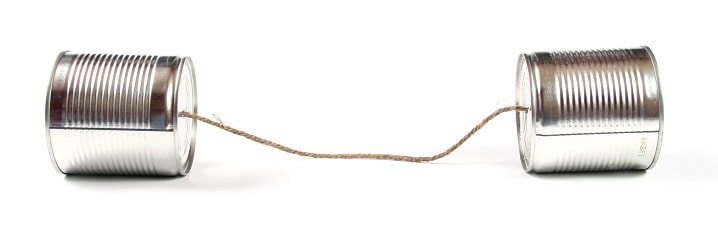
\includegraphics[scale=0.42]{tin-can-telephone.jpg}
  \end{center}
\end{frame}

\begin{frame}{Communiquer avec du bruit ?}
  \begin{center}
  \begin{tikzpicture}
    %%% Tin can telephone %%%
    \node at (4.7,0) (tin) {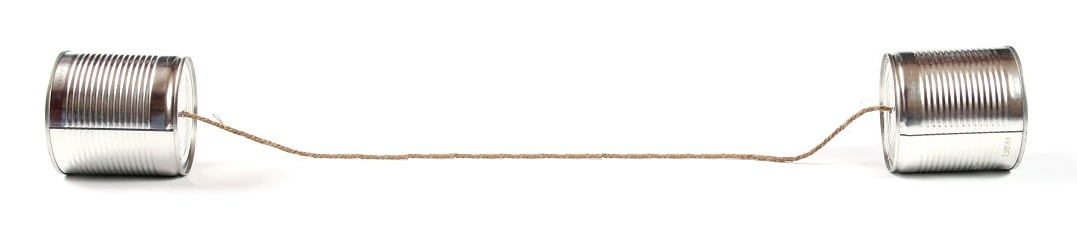
\includegraphics[scale=0.22]{long-tin-can-telephone.jpg}};

    %%% Left callouts %%%
    \only<1-2>{\node[ellipse callout, draw, callout relative pointer={(-0.3,-0.3)}] at (-0.1,0.1) (Alice) {\Large Allô!};}
    \only<3>{\node[ellipse callout, draw, callout relative pointer={(-0.3,-0.3)}] at (-0.1,2.1) (Alice) {\Large \alert{A}llô!};
      \node[ellipse callout, draw, callout absolute pointer={(-0.1,1.5)}, text=blue] at (-0.1,0.1) (Alice) {Alfa};}
    \only<4>{\node[ellipse callout, draw, callout relative pointer={(-0.3,-0.3)}] at (-0.1,2.1) (Alice) {\Large A\alert{l}lô!};
      \node[ellipse callout, draw, callout absolute pointer={(-0.1,1.5)}, text=blue] at (-0.1,0.1) (Alice) {Lima};}
    \only<5>{\node[ellipse callout, draw, callout relative pointer={(-0.3,-0.3)}] at (-0.1,2.1) (Alice) {\Large Al\alert{l}ô!};
      \node[ellipse callout, draw, callout absolute pointer={(-0.1,1.5)}, text=blue] at (-0.1,0.1) (Alice) {Lima};}
    \only<6>{\node[ellipse callout, draw, callout relative pointer={(-0.3,-0.3)}] at (-0.1,2.1) (Alice) {\Large All\alert{ô}!};
      \node[ellipse callout, draw, callout absolute pointer={(-0.1,1.5)}, text=blue] at (-0.1,0.1) (Alice) {\small Oscar};}
    %%% Cloud %%%
    \only<1>{\node at (4.6,1.5) (wcloud) {
\includegraphics[scale=0.3]{rcloud_white.png}};}
    \only<2-6>{\node at (4.6,1.5) (cloud) {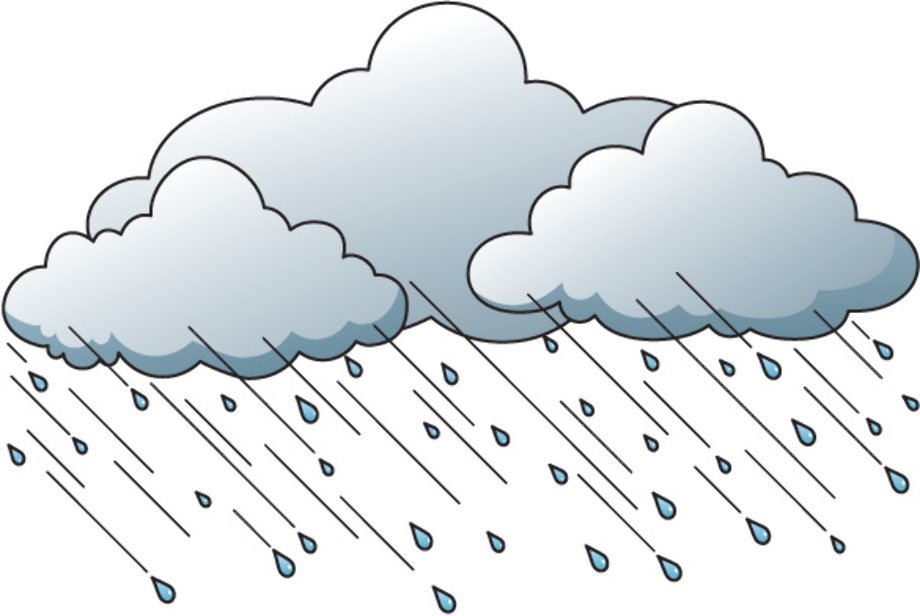
\includegraphics[scale=0.3]{rcloud.png}};}

    %%% Right callouts %%%
    \only<1>{\node[ellipse callout, draw, callout relative pointer={(-0.2,0)}] at (9.7,0.1) (Bob) {\Large Allô!};}
    \only<2>{\node[dashed, ellipse callout, draw, callout relative pointer={(-0.2,0)}] at (9.7,0.1) (Bob) {\tiny Ah, l'eau!};}
    \only<3>{\node[dashed, ellipse callout, draw, callout relative pointer={(-0.2,0)}, text=blue] at (9.4,0.1) (Bob) {\tiny Alma};
      \node[ellipse callout, draw, callout absolute pointer={(9.4,0.5)}] at (9.4,2.1) (Alice) {\Large \alert{A}};}
    \only<4>{\node[dashed, ellipse callout, draw, callout relative pointer={(-0.2,0)}, text=blue] at (9.4,0.1) (Bob) {\tiny Lena};
      \node[ellipse callout, draw, callout absolute pointer={(9.4,0.5)}] at (9.4,2.1) (Alice) {\Large A\alert{L}};}
    \only<5>{\node[dashed, ellipse callout, draw, callout relative pointer={(-0.2,0)}, text=blue] at (9.4,0.1) (Bob) {\tiny Rima};
      \node[ellipse callout, draw, callout absolute pointer={(9.4,0.5)}] at (9.4,2.1) (Alice) {\Large AL\alert{L}};}
    \only<6>{\node[dashed, ellipse callout, draw, callout relative pointer={(-0.2,0)}, text=blue] at (9.5,0.1) (Bob) {\tiny Lascar};
      \node[ellipse callout, draw, callout absolute pointer={(9.5,0.5)}] at (9.5,2.1) (Alice) {\Large ALL\alert{O}};}
  \end{tikzpicture}
  \end{center}
\end{frame}


\begin{frame}{Modélisation mathématique}
  \begin{center}
    \begin{tikzpicture}[auto, node distance=2cm,>=latex']
      \node [bigblock] (W) {\only<1-2>{$W$}\only<3>{$6/10$}\only<4>{$3/10$}\only<5>{$1/10$}};
      \node [right of=W] (y) {\only<1-2>{$y$}\only<3>{\emph{alfa}}\only<4>{\emph{alma}}\only<5>{\emph{alvo}}};
      \node [left of=W] (x) {\only<1-2>{$x$}\only<3-5>{\emph{alfa}}};
      \draw [->] (x) -- (W);
      \draw [->] (W) -- (y);
    \end{tikzpicture}

    \pause
    \bigskip
    Probabilité \only<2>{$W(y|x)$}\only<3>{$6/10$}\only<4>{$3/10$}\only<5>{$1/10$} d'avoir la sortie \only<2>{$y$}\only<3>{\emph{alfa}}\only<4>{\emph{alma}}\only<5>{\emph{alvo}} pour l'entrée \only<2>{$x$}\only<3-5>{\emph{alfa}}
  \end{center} 
\end{frame}

\begin{frame}{Le problème du codage de canal}
  \begin{center}
    \begin{tikzpicture}[auto, node distance=2.5cm,>=latex']
      \node [block] (e) {$e$};
      \node [bigblock, right of=e] (W) {\only<1,5>{$W$}\only<2>{$6/10$}\only<3>{$3/10$}\only<4>{$1/10$}};
      \node [block, right of=W] (d) {$d$};
      \draw [->] (e) -- node[name=x, text=blue] {\only<1,5>{$x$}\only<2-4>{\emph{alfa}}} (W);
      \draw [->] (W) -- node[name=y, text=blue] {\only<1,5>{$y$}\only<2>{\emph{alfa}}\only<3>{\emph{alma}}\only<4>{\emph{alvo}}} (d);
      \node [left of=e, node distance=1.5cm, text=red] (i) {\only<1>{$i$}\only<2-4>{a}\only<5>{a,\ldots,z}};
      \node [right of=d,  node distance=1.5cm, text=red] (j) {\only<1>{$j$}\only<2-3>{a}\only<4>{b}\only<5>{a,\ldots,z}};
      \draw [draw,->] (i) -- (e);
      \draw [draw,->] (d) -- (j);
    \end{tikzpicture}

    \bigskip

    Trouver $e$ et $d$ qui maximise la probabilité d'avoir \alert{$j=i$}\only<5>{\ldots\\
      \bigskip
      \ldots sur tout l'alphabet (noté $[k]$; ici $k=26$) !
      \[ \text{\underline{Formellement:} } \underset{e,d}{\max} \ \frac{1}{k} \sum_{i,x,y} e(x|i)W(y|x)d(i|y) \]
    }
  \end{center}
\end{frame}

\begin{frame}{Résolution \cite{BF18}}
  \begin{itemize}
  \item \underline{Objectif:} méthode systématique (algorithme) pour trouver les meilleurs $e,d$ pour un $W$.
    \pause
  \item \underline{Problème:} impossible (\textrm{NP}-difficulté) d'élaborer un algorithme efficace (temps polynomial) qui trouve ces $e,d$.
    \bigskip
    \pause
  \item \underline{Solution:} plutôt que les meilleurs $e,d$, on se contente d'un choix de $e,d$ avec une valeur \emph{proche} des meilleurs.
    
    \pause
    \bigskip

  \item \cite{BF18}: approximation qui garantit au moins $\simeq 63\%$ ($1-e^{-1}$) aussi bien que les meilleurs.
  \item Impossible (\textrm{NP}-difficile) de faire mieux que $1-e^{-1}$.
  \end{itemize}
\end{frame}

\begin{frame}{Décodage de liste}
  \begin{center}
    \begin{tikzpicture}[auto, node distance=2.5cm,>=latex']
      \node [block] (e) {$e$};
      \node [bigblock, right of=e] (W) {\only<1,3-6>{$W$}\only<2>{$1/10$}};
      \node [block, right of=W] (d) {$d$};
      \draw [->] (e) -- node[name=x] {\only<1,3-6>{\textcolor{blue}{$x$}}\only<2>{\textcolor{blue}{\emph{alfa}}}} (W);
      \draw [->] (W) -- node[name=y] {\only<1,3-6>{\textcolor{blue}{$y$}}\only<2>{\textcolor{blue}{\emph{alvo}}}} (d);
      \node [left of=e, node distance=1.5cm] (i) {\only<1,3-6>{\alert{$i$}}\only<2>{\alert{a}}};
      \node [right of=d,  node distance=2cm] (j) {\only<1>{\alert{$[j_1,j_2]$}}\only<2>{\alert{[a,b]}}\only<3-6>{\alert{$[j_1,j_2,\ldots,j_{\ell}]$}}};
      \draw [draw,->] (i) -- (e);
      \draw [draw,->] (d) -- (j);
    \end{tikzpicture}

    \bigskip
    Trouver $e,d$ qui maximise la probabilité que \only<1-2>{\alert{$j_1$ ou $j_2$}}\only<3-6>{\alert{$j_1,j_2,\ldots$ ou $j_{\ell}$}} égal à \alert{$i$}.
  \end{center}
  
  \pause\pause\pause
  
  \begin{itemize}
  \item \cite{BFGG20}: Algorithme d'approximation avec un facteur $1-\frac{\ell^{\ell}e^{-\ell}}{\ell!}$ (pour $\ell=2$, correspond à $\simeq 73\%$).
    \pause
  \item On va montrer que c'est \textrm{NP}-difficile de faire mieux.
    \pause
  \item On va étudier une généralisation, où la taille $\ell$ de la liste n'est pas fixée, mais vient avec une pénalité $\frac{\varphi(\ell)}{\ell}$.
  \end{itemize}
\end{frame}

\subsection{Les corrélations non-signalantes}
\begin{frame}{La physique quantique\only<3>{\ldots et ses idées reçues}}
  \begin{center}
    \pause
  \begin{tikzpicture}
    %%% Tin can telephone %%%
    \node at (0,0) (cat_ud) {
\includegraphics[scale=0.1]{cat.png}};
    \node[rotate=180] at (5,0) (cat_ud) {
\includegraphics[scale=0.1]{cat.png}};
    \node[scale=0.5, align=center, ellipse callout, draw, fill=white, callout relative pointer={(0.7,-0.3)}] at (-0.1,0) (upside) {J'ai la tête\\ en bas.};
    \node[scale=0.5, align=center, ellipse callout, draw, fill=white, callout relative pointer={(-0.7,0.3)}] at (5.1,0) (upside) {J'ai la tête\\ en haut.};

    \only<2>{\node at (2.5,-3.5) (cat_q) {
\includegraphics[scale=0.12]{cat_question_white.png}};}
    \only<3>{\node at (2.5,-3.5) (cat_q) {
\includegraphics[scale=0.12]{cat_question.png}};
      \node[scale=0.5, align=center, ellipse callout, draw, fill=white, callout relative pointer={(0.6,-0.6)}] at (2.7,-2.4) (Notallowed) {J'ai rien\\ à faire là!};
    }
  \end{tikzpicture}
  \end{center}
\end{frame}

\begin{frame}{De quoi parle la physique quantique ?}
  \begin{itemize}
  \item Comprendre physique à l'\emph{échelle} des atomes -- \emph{un million de fois plus petit qu'un grain de sable !} (0,1nm)
    \begin{center}
      \begin{tikzpicture}
        \node at (0,0) (atom1) {
\includegraphics[scale=0.04]{atom.jpg}};
        \node at (3,0) (atom2) {
\includegraphics[scale=0.04]{atom.jpg}};
        \only<3-4>{\draw[snake=coil, segment aspect=0, draw=blue] (0,0) -- (3,0);}
      \end{tikzpicture}
    \end{center}
    \pause
  \item Phénomène spécifique à cette échelle...\pause \textcolor{blue}{l'intrication quantique :}
    \pause
    \\ \ 
    \begin{center}
      \alert{Deux particules \emph{corrélées} à très grande distance\\
      \emph{Inexplicable} par physique non quantique !}
    \end{center}
  \end{itemize}
\end{frame}

\begin{frame}{Le paradoxe Einstein-Podolski-Rosen}

  \begin{itemize}
  \item \underline{Années 1920 :} naissance de la physique quantique
    \pause
    \bigskip
  \item \underline{Paradoxe EPR~\cite{EPR35} :} deux particules intriquées à distance
    \begin{center}
      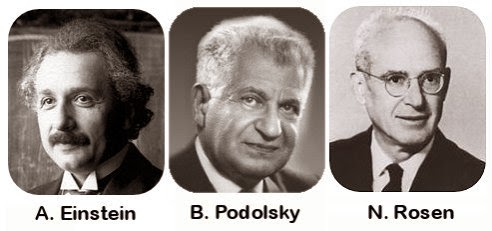
\includegraphics[scale=0.3]{EPR.jpg}
    \end{center}
    \pause
    \begin{enumerate}
    \item Soit contradiction avec le \emph{principe de localité}
    \item Soit mécanique quantique \emph{incomplète} (variables cachées)
    \end{enumerate}
    \pause
  \item De manière inattendue, c'est \alert{le premier} qui décrit la réalité !
  \item Communication plus rapide que la lumière ? \pause{\textcolor{blue}{\emph{Non, corrélations !}}}
  \end{itemize}
\end{frame}

\begin{frame}{Inégalités de Bell et expérience d'Aspect}
  \begin{itemize}
  \item \underline{Inégalités de Bell~\cite{Bell64} :} expérience distinguant corrélations :\begin{enumerate}
    \item causées par de l'intrication quantique
    \item provenant de variables cachées
  \end{enumerate}
  \end{itemize}
  \pause
  \begin{columns}
    \begin{column}{2cm}
      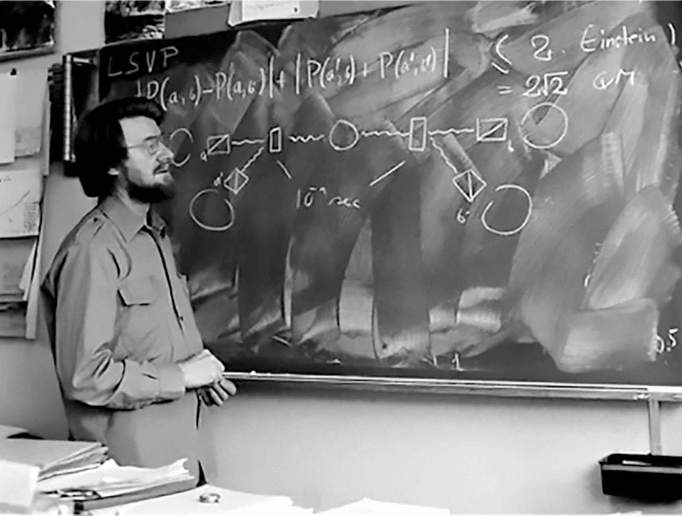
\includegraphics[scale=0.15]{BellAspect.png}
    \end{column}
    \begin{column}{6cm}
      \begin{itemize}
      \item \underline{Expérience d'Aspect~\cite{ADG82} :} réalisation pratique de cette expérience.
      \end{itemize}
    \end{column}
    \end{columns}
    \pause
    \bigskip
    \begin{itemize}
  \item \underline{Expérience QUESS~\cite{Yin17} :} intrication entre particules à 1200 km de distance
  \end{itemize}
\end{frame}

\begin{frame}{Le jeu CHSH}
  \begin{center}
    \only<2->{On tire $x,y$ au hasard dans $\{0,1\}$, on les donne à Alice et Bob.\\}
    \bigskip
   \begin{tikzpicture}[auto, node distance=1.8cm,>=latex']
      \node [block] (A) {
\includegraphics[scale=0.08]{Alice.png}};
      \only<2->{\node [above of=A] (x) {$x$};
      \draw [->] (x) -- (A);}
      \only<3->{\node [below of=A] (a) {\only<3-6>{$\alert{a}$}\only<7>{\textcolor{darkgreen}{$\mathcal{A}(x)=0$}}};
      \draw [->] (A) -- (a);}

      \node [right of=A] (I) {};
      \only<4->{\node [color=blue,above of=I,outer sep=0pt,circle,fill,inner sep=1pt] (Iabove) {};
      \node [color=blue,below of=I,outer sep=0pt,circle,fill,inner sep=1pt] (Ibelow) {};
      \draw [color=blue,dotted, thick] (Iabove) -- (Ibelow);}
      
      \node [block, right of=I] (B) {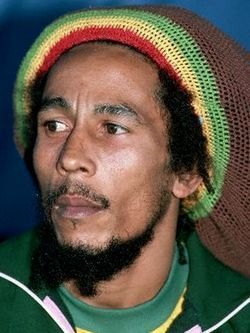
\includegraphics[scale=0.16]{Bob.jpg}};
      \only<2->{\node [above of=B] (y) {$y$};
      \draw [->] (y) -- (B);}
      \only<3->{\node [below of=B] (b) {\only<3-6>{$\alert{b}$}\only<7>{\textcolor{darkgreen}{$\mathcal{B}(y)=0$}}};
      \draw [->] (B) -- (b);}

      \only<7>{\node [starburst, fill=white, draw=darkgreen, line width=1pt, text=darkgreen] at (I) {\Large $3/4$};}
   \end{tikzpicture}
   \bigskip
   \\
   \only<3-4>{Alice et Bob choisissent $\alert{a}$ et $\alert{b}$ dans $\{0,1\}$\only<4->{, \textcolor{blue}{sans communiquer !}}\\\bigskip}
   \only<5->{\underline{Objectif :} Si $x=y=1$, alors $\alert{a}\not=\alert{b}$ ; sinon $\alert{a}=\alert{b}$.\\\bigskip}
   \only<6->{\large\emph{Quelle est la probabilité de succès de la meilleure stratégie ?}}
  \end{center}
\end{frame}

\begin{frame}{Variables cachées, intrication quantique et non-signalante}
  \begin{center}
    Et si Alice et Bob partagent\ldots\only<2-4>{des \textcolor{blue}{\emph{variables cachées}} ?}\only<5-7>{de \textcolor{blue}{\emph{l'intrication quantique}} ?}\only<8->{des \textcolor{blue}{\emph{corrélations non-signalantes}} ?}\\\bigskip
    \begin{tikzpicture}[auto, node distance=1.8cm,>=latex']
      \node [block] (A) {
\includegraphics[scale=0.08]{Alice.png}};
      \node [above of=A] (x) {$x$};
      \draw [->] (x) -- (A);
      \node [below of=A] (a) {$\alert{a}$};
      \draw [->] (A) -- (a);

      \node [right of=A] (I) {};
      \node [color=blue,above of=I,outer sep=0pt,circle,fill,inner sep=1pt] (Iabove) {};
      \node [color=blue,below of=I,outer sep=0pt,circle,fill,inner sep=1pt] (Ibelow) {};
      \draw [color=blue,dotted, thick] (Iabove) -- (Ibelow);
      
      \node [block, right of=I] (B) {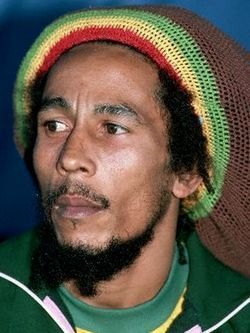
\includegraphics[scale=0.16]{Bob.jpg}};
      \node [above of=B] (y) {$y$};
      \draw [->] (y) -- (B);
      \node [below of=B] (b) {$\alert{b}$};
      \draw [->] (B) -- (b);

      \only<2->{
        \draw [snake=coil,segment aspect=0, draw=blue] (A) -- (B);
        \node [circle, fill=white, draw=blue, text=blue] at (I) (Corr) {\only<2-4>{$\lambda$}\only<5-7>{$\varphi$}\only<8->{\textrm{NS}}};}
      \only<4>{\node [starburst, fill=white, draw=darkgreen, line width=1pt, text=darkgreen] at (I) {\Large $3/4$};}
      \only<7>{\node [starburst, fill=white, draw=darkgreen, line width=1pt, text=darkgreen] at (I) {\Large $85\%$};}
      \only<11>{\node [starburst, fill=white, draw=darkgreen, line width=1pt, align=left, text=darkgreen] at (I) {\Large $100\%$};}
    \end{tikzpicture}\\\bigskip
    
    \only<3-4>{\emph{Avant l'expérience}, s'accordent sur un \textcolor{blue}{$\lambda$} aléatoire.\\
      Alice et Bob peuvent l'utiliser \emph{tous les deux} pour choisir $\alert{a}$ et $\alert{b}$.}
    \only<6-7>{Toujours \textcolor{blue}{pas de communication} ! Stratégie $P(\alert{ab}\textcolor{blue}{\textbf{|}}xy)$ vérifie que :\\
      $\alert{a}$ \textcolor{blue}{ne dépend pas de} $y$ et $\alert{b}$ \textcolor{blue}{ne dépend pas de} $x$.}
    \only<9-10>{\emph{Toutes les stratégies $P(\alert{ab}\textcolor{blue}{\textbf{|}}xy)$ \textcolor{blue}{sans communication}}, càd telles que :\\}
    \only<9>{$\alert{a}$ \textcolor{blue}{ne dépend pas de} $y$ et $\alert{b}$ \textcolor{blue}{ne dépend pas de} $x$.}
    \only<10>{$P(\alert{a}|xy)=P(\alert{a}|xy')$ et $P(\alert{b}|xy)=P(\alert{b}|x'y)$.}
    \only<11->{\textcolor{darkgreen}{$P(ab|xy) = \frac{1}{2}$ si $a,b,x,y$ satisfont l'objectif, $P(ab|xy) = 0$ sinon.\\ Du point de vue d'Alice, $P(a|xy) = \frac{1}{2}$, indépendant de $y$!}}
  \end{center}
\end{frame}

\begin{frame}{Assistance non-signalante pour le codage de canal}
  \begin{center}
    \begin{tikzpicture}[auto, node distance=1.6cm,>=latex']
      \only<1>{\node [bigblock] (W) {$W$};
        \node [left of=W] (x) {$x$};
        \node [block,left of=x] (e) {$e$};
        \node [left of=e] (i) {$i$};
        \node [right of=W] (y) {$y$};
        \node [block,right of=y] (d) {$d$};
        \node [right of=d] (j) {$j$};
        \draw [->] (i) -- (e);
        \draw [->] (e) -- (x);
        \draw [->] (x) -- (W);
        \draw [->] (W) -- (y);
        \draw [->] (y) -- (d);
        \draw [->] (d) -- (j);}

      \only<2->{\node [block] (A) {$e$};
      \node [above of=A] (x) {$i$};
      \draw [->] (x) -- (A);
      \node [below of=A] (a) {\only<2>{$x$}\only<3->{$\alert{x}$}};
      \draw [->] (A) -- (a);

      \node [right of=A] (I) {};
      
      \node [block, right of=I] (B) {$d$};
      \node [above of=B] (y) {$y$};
      \draw [->] (y) -- (B);
      \node [below of=B] (b) {\only<2>{$j$}\only<3->{$\alert{j}$}};
      \draw [->] (B) -- (b);
      
      \node [dashed,right of=B] (Bright) {};
      \node [dashed,bigblock,right of=Bright] (W) {$W$};
      \draw [dashed,->] (a) to[out=-20,in=-90] (W);
      \draw [dashed,->] (W) to[out=90,in=20] (y);}

      
      \only<3->{\node [color=blue,above of=I,outer sep=0pt,circle,fill,inner sep=1pt] (Iabove) {};
      \node [color=blue,below of=I,outer sep=0pt,circle,fill,inner sep=1pt] (Ibelow) {};
      \draw [color=blue,dotted, thick] (Iabove) -- (Ibelow);
      \draw [snake=coil,segment aspect=0, draw=blue] (A) -- (B);
      \node [circle, fill=white, draw=blue, text=blue] at (I) (Corr) {\textrm{NS}};}
    \end{tikzpicture}\\
    \only<2>{On peut considérer la stratégie encodage-décodage indépendamment de $W$ !}
    \only<3>{La stratégie encodage-décodage est décrite par $P(\alert{xj}\textcolor{blue}{\textbf{|}}iy)$ :\\
      Calcul de $e(\alert{x}|i)$ \textcolor{blue}{sans} $y$ ; corrélation \emph{\alert{globale}} inexplicable \emph{localement}.}
    \only<4>{\underline{\cite{BF18} :}  meilleure communication (jusqu'à $58\%$ ($\frac{e^{-1}}{1-e^{-1}}$)), mais pas de changement de \emph{capacité} du canal.}
  \end{center}
\end{frame}

\begin{frame}{Canaux en réseau}
  \begin{center}
      \begin{tikzpicture}[auto, node distance=2cm,>=latex']
        \only<1>{\node (W) {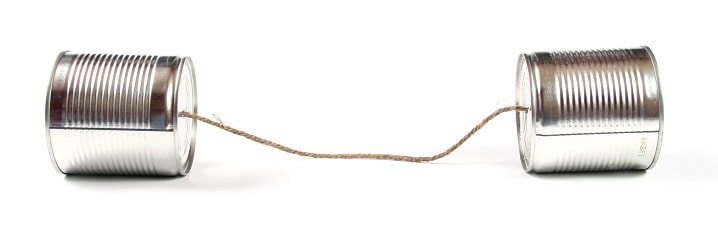
\includegraphics[scale=0.3]{tin-can-telephone.jpg}};
          %\node [right of=W] (y) {$y$};
          %\node [left of=W] (x) {$x$};
          %\draw [->] (x) -- (W);
          %\draw [->] (W) -- (y);
          \node [below of=W] (txt) {Ne modélise pas les situations à plus de deux parties !};}

        \only<2>{\node (Wa) {};
          \node [above right of=Wa] (y1) {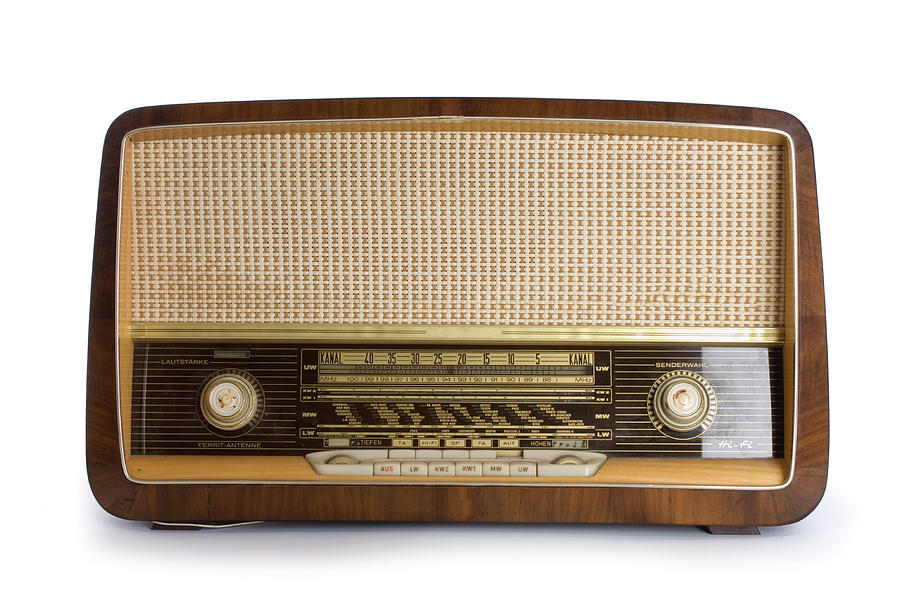
\includegraphics[scale=0.2]{radio.jpg}};
          \node [below right of=Wa] (y2) {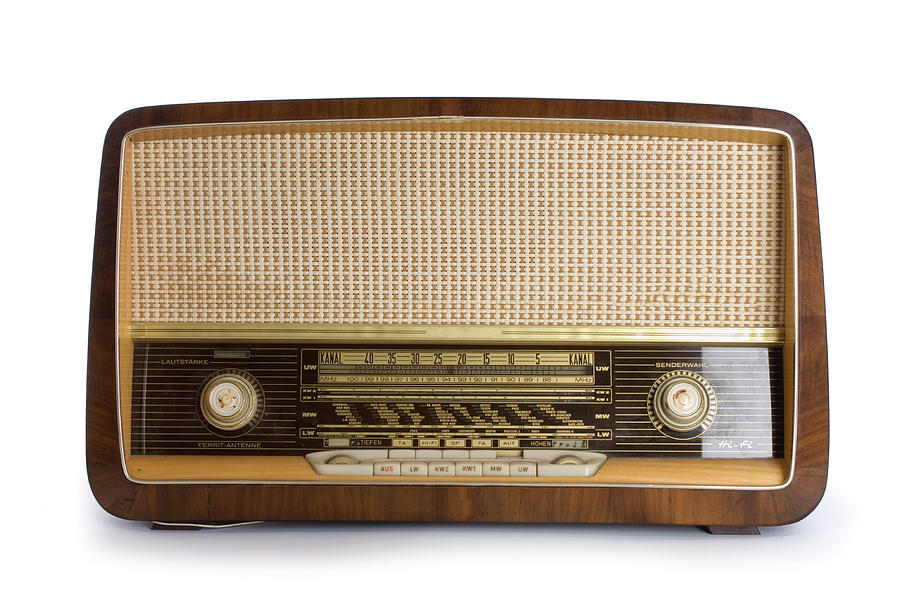
\includegraphics[scale=0.2]{radio.jpg}};
          \node [left of=Wa] (x) {
\includegraphics[scale=0.012]{france_inter.png}};
          \node [rotate=-70] (signal1a) at ($(x)!0.48!(y1)$) {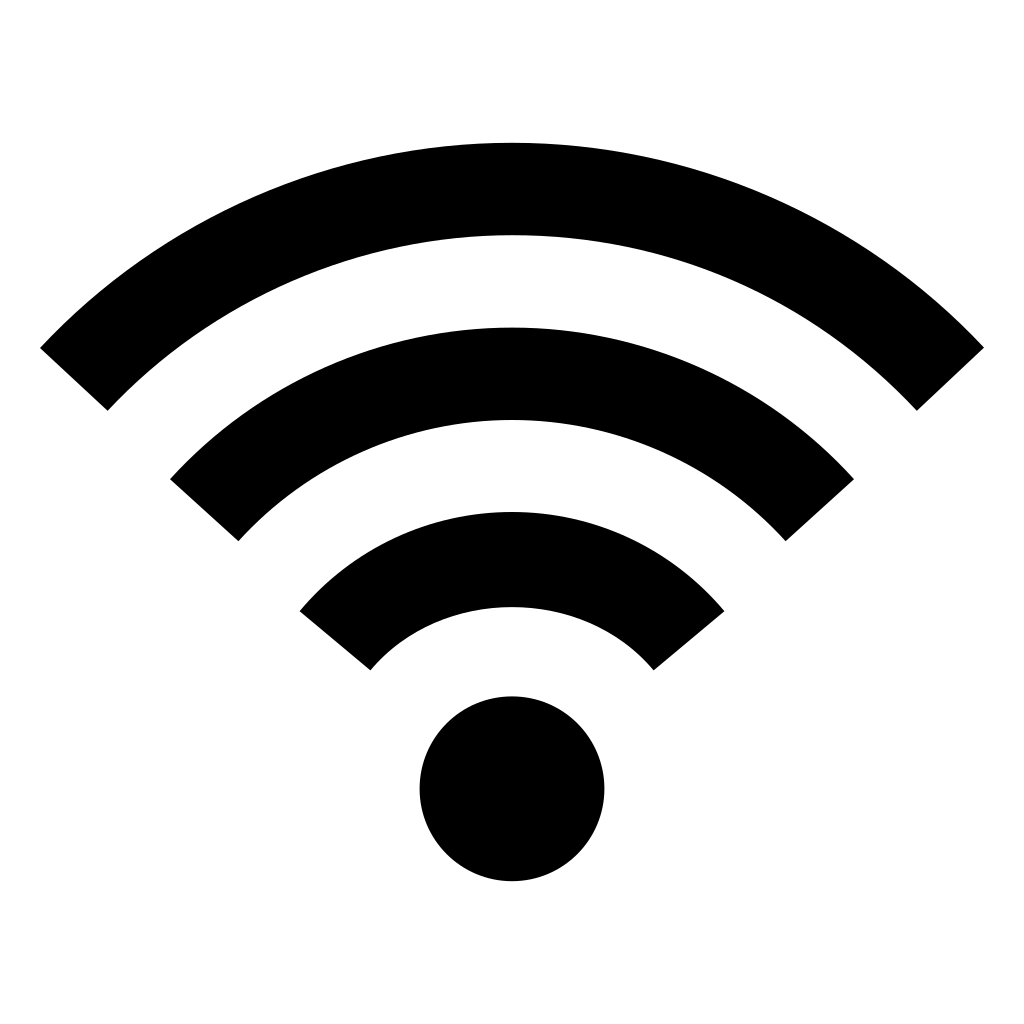
\includegraphics[scale=0.1]{signal.png}};
          \node [rotate=-110] (signal2a) at ($(x)!0.48!(y2)$) {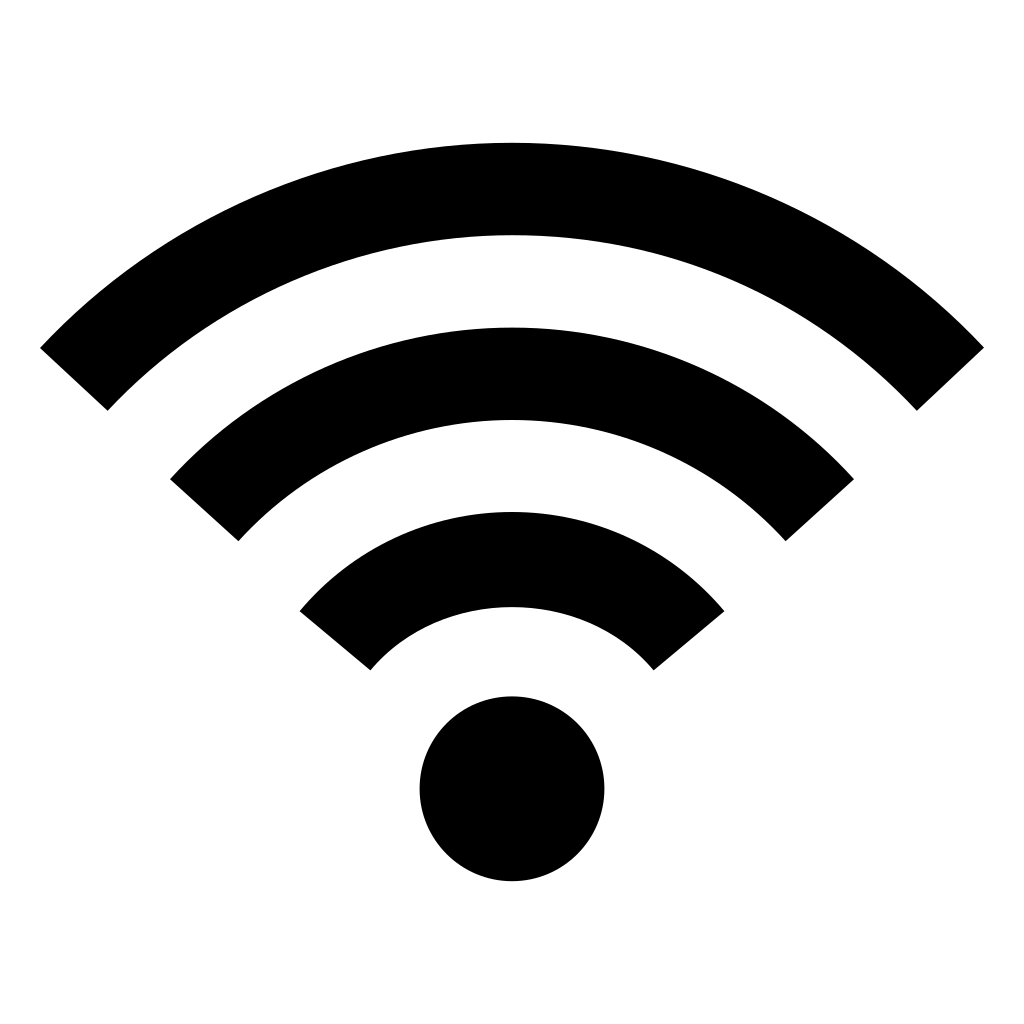
\includegraphics[scale=0.1]{signal.png}};
          \node [below of=signal2a] (txta) {Canal de diffusion};

          \node [right of=Wa] (pos1) {};
          \node [right of=pos1] (pos2) {};
          \node [right of=pos2] (Wb) {};
          \node [right of=Wb] (y) {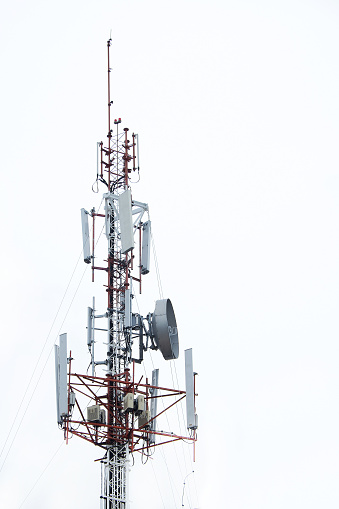
\includegraphics[scale=0.7]{antenne.jpg}};
          \node [above left of=Wb] (x1) {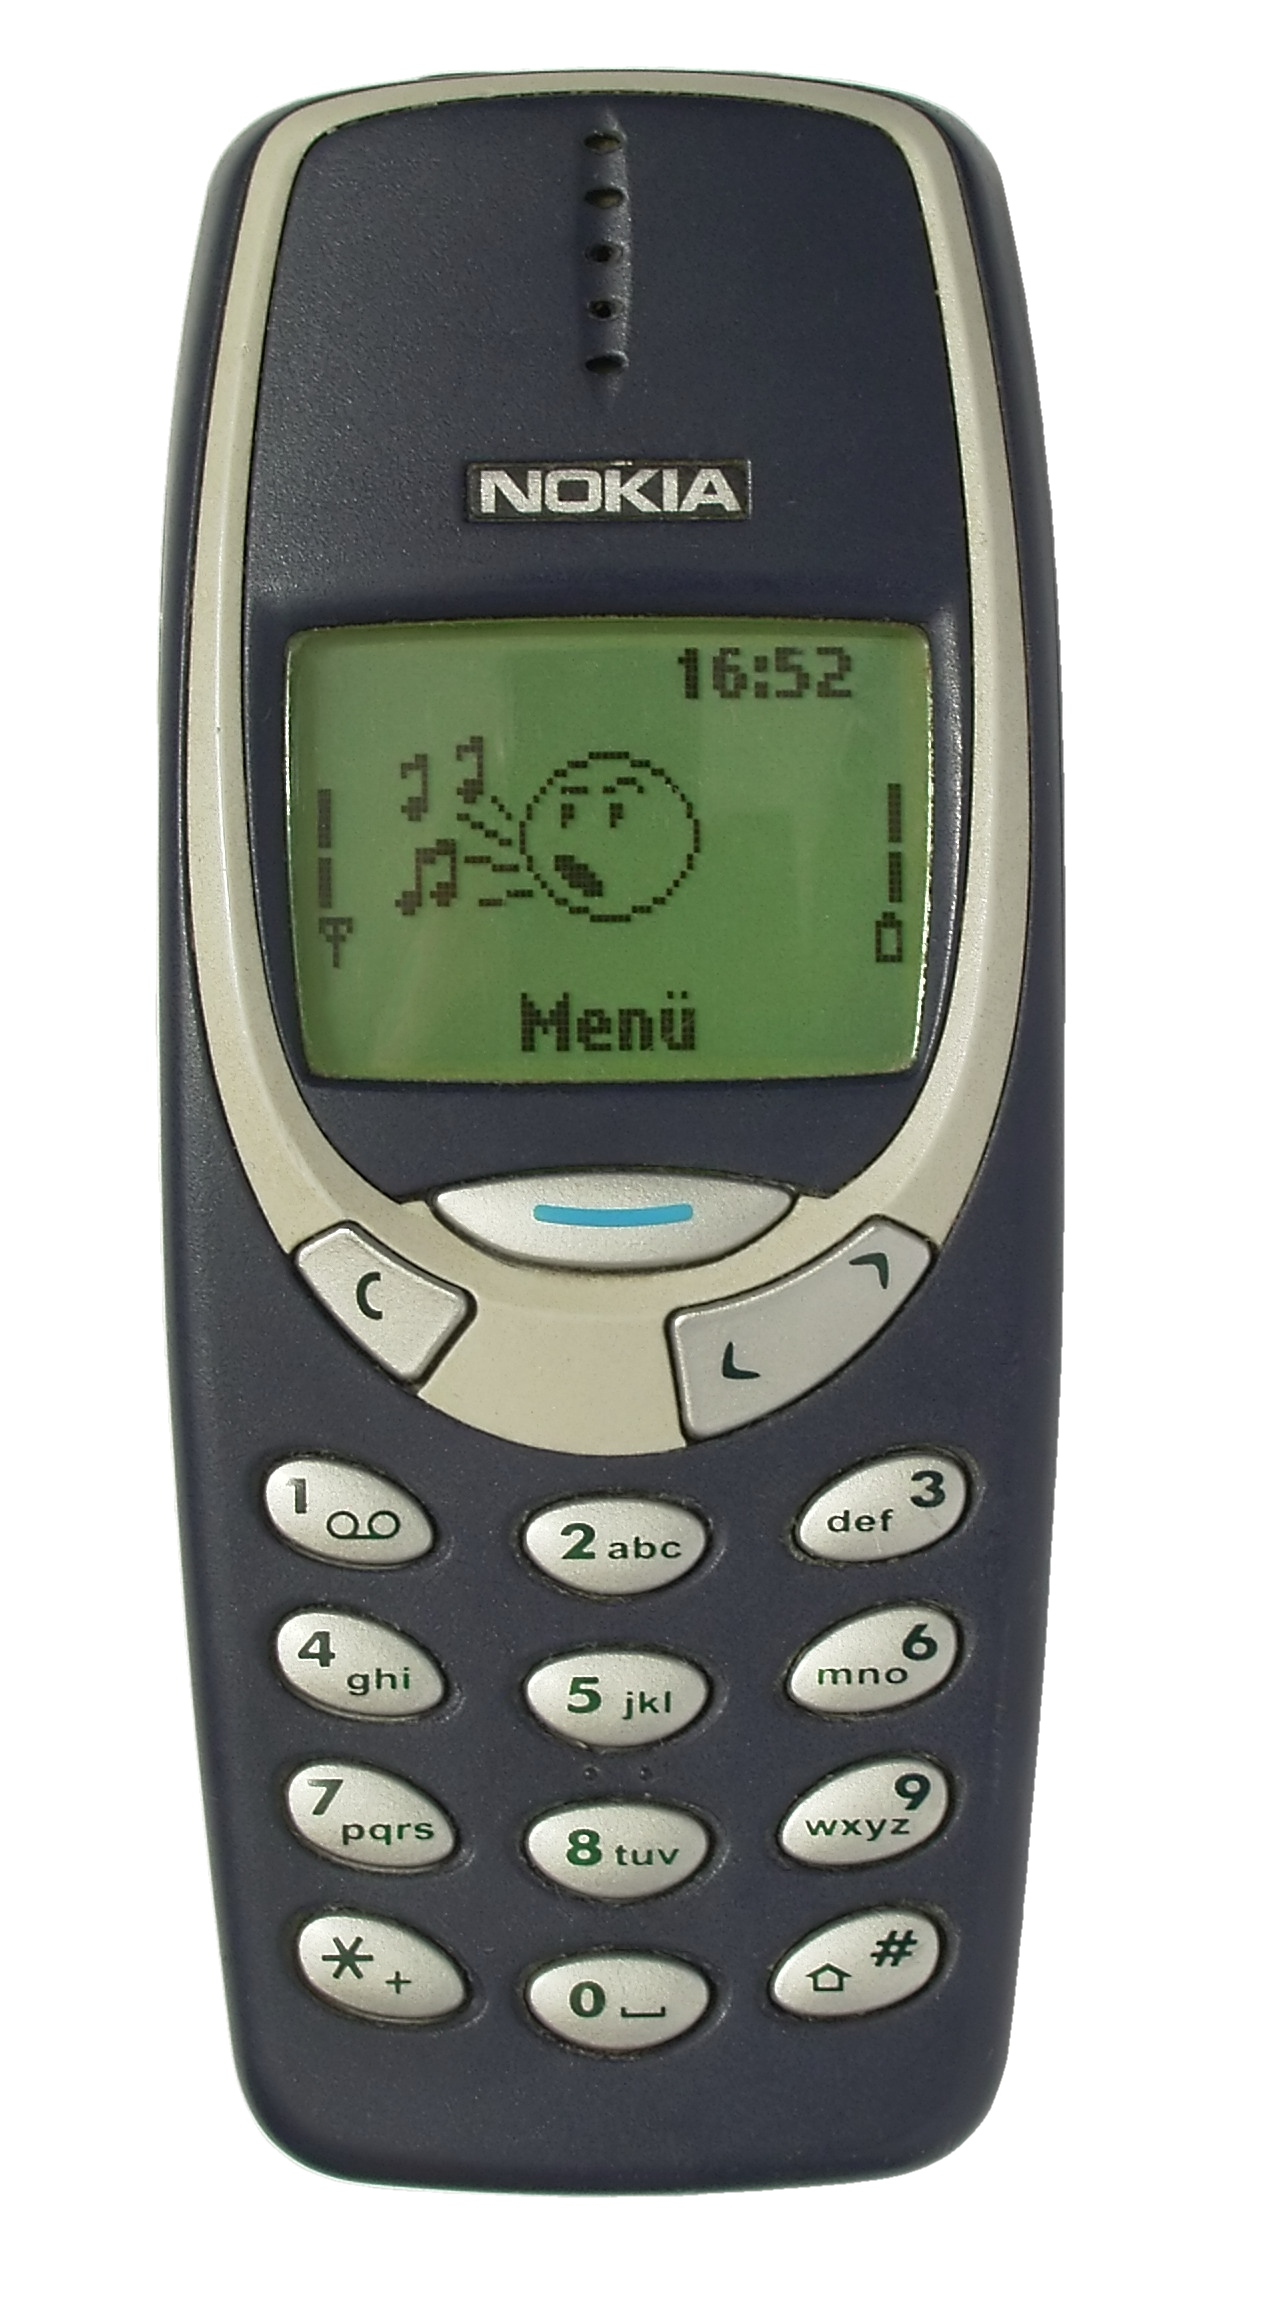
\includegraphics[scale=0.015]{phone.jpg}};
          \node [below left of=Wb] (x2) {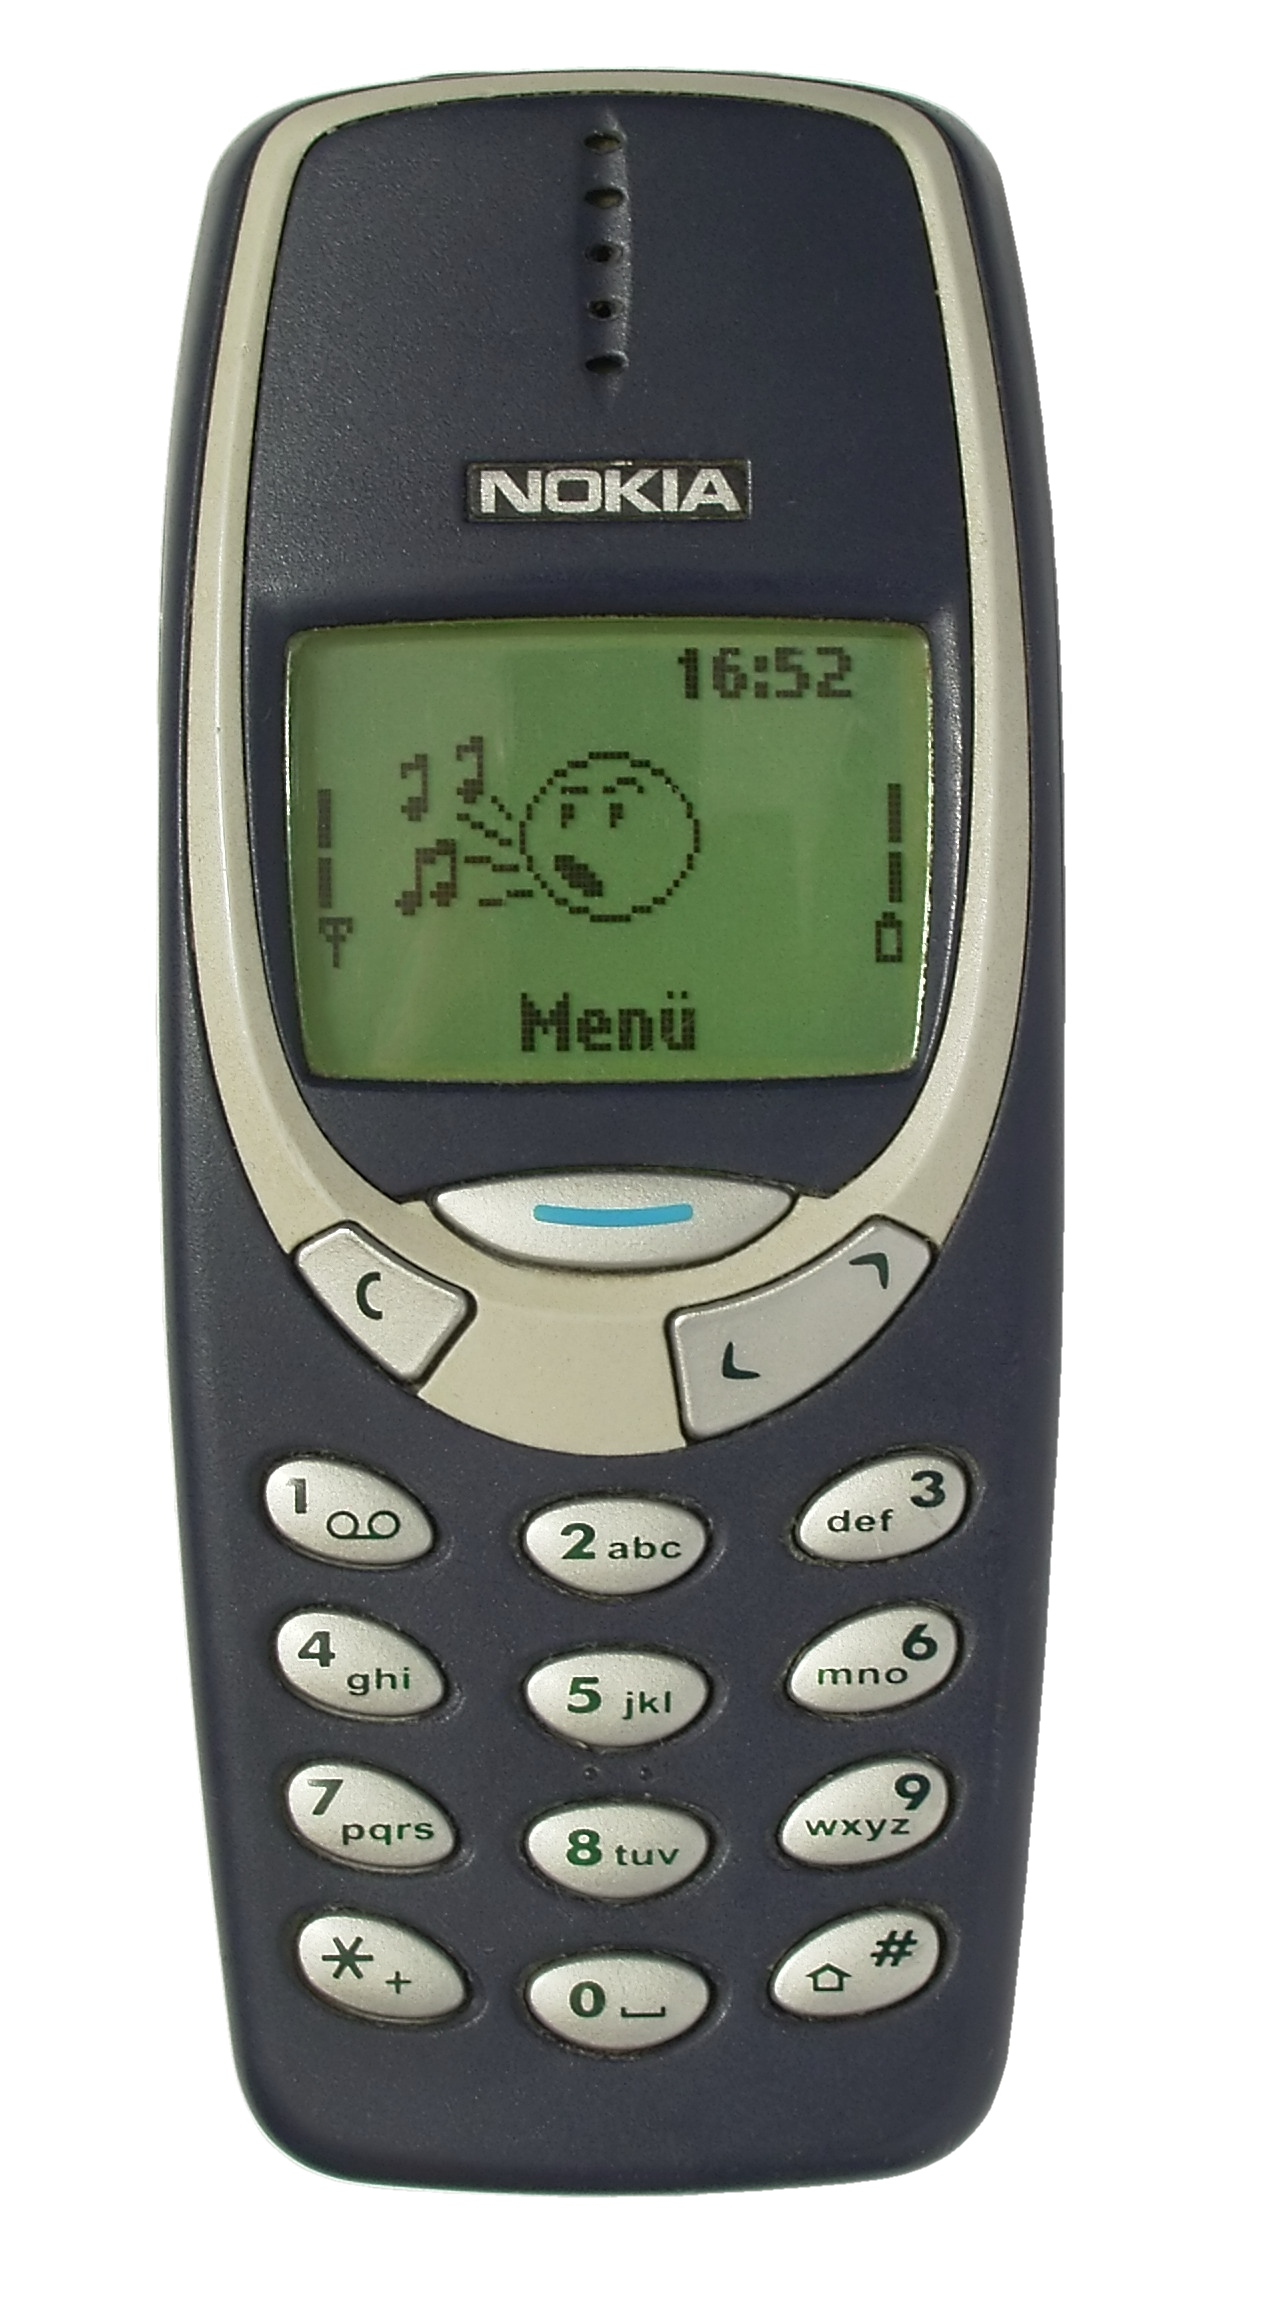
\includegraphics[scale=0.015]{phone.jpg}};
          \node [rotate=-110] (signal1b) at ($(x1)!0.45!(y)$) {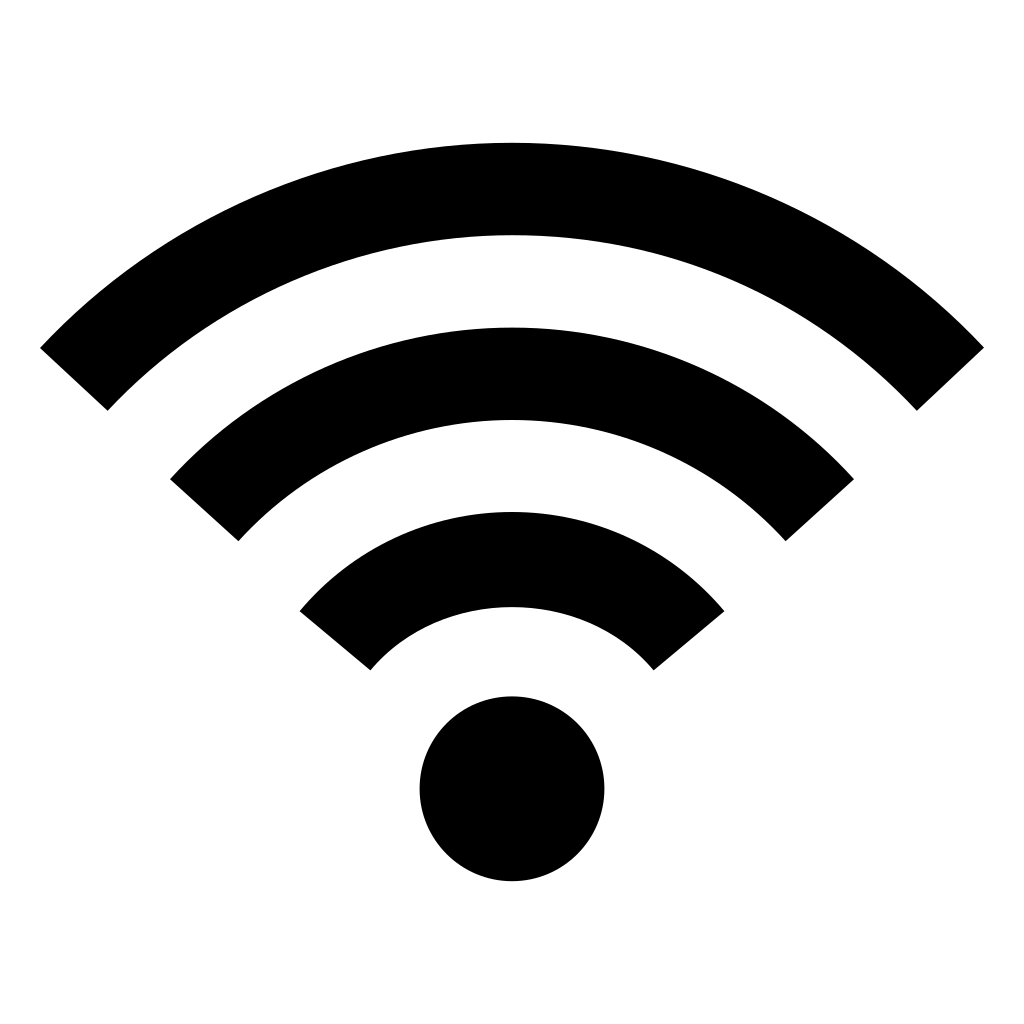
\includegraphics[scale=0.1]{signal.png}};
          \node [rotate=-70] (signal2b) at ($(x2)!0.45!(y)$) {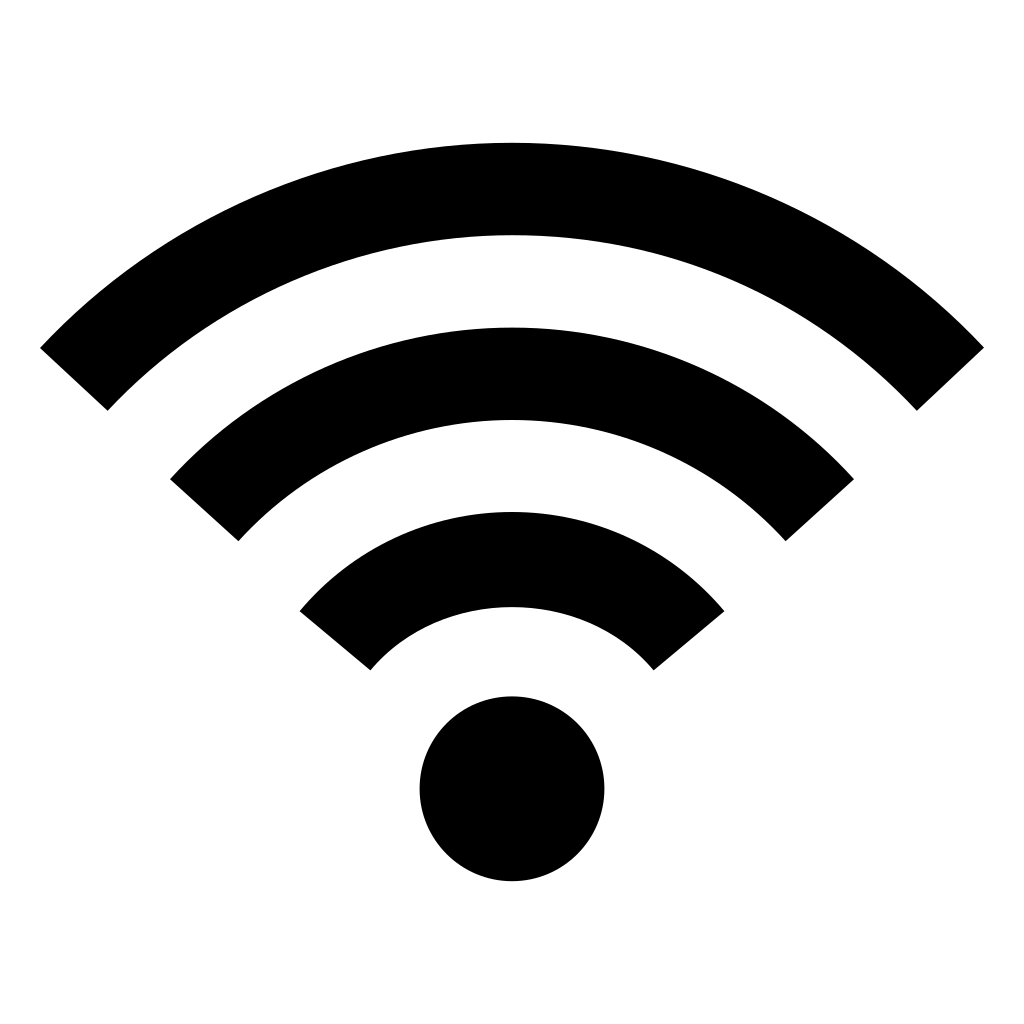
\includegraphics[scale=0.1]{signal.png}};
          \node [below of=signal2b] (txt) {Canal à accès multiple};}

        \only<3->{\node [bigblock] (Wa) {$W$};
          \node [above right of=Wa] (y1) {$y_1$};
          \node [below right of=Wa] (y2) {$y_2$};
          \node [left of=Wa] (x) {$x$};
          \draw [->] (x) -- (Wa);
          \draw [->] (Wa) -- (y1);
          \draw [->] (Wa) -- (y2);
          \node [below of=Wa] (txta) {Canal de diffusion};

          \node [right of=Wa] (pos1) {};
          \node [right of=pos1] (pos2) {};
          \node [bigblock, right of=pos2] (Wb) {$W$};
          \node [right of=Wb] (y) {$y$};
          \node [above left of=Wb] (x1) {$x_1$};
          \node [below left of=Wb] (x2) {$x_2$};
          \draw [->] (x1) -- (Wb);
          \draw [->] (x2) -- (Wb);
          \draw [->] (Wb) -- (y);
          \node [below of=Wb] (txt) {Canal à accès multiple};}
      \end{tikzpicture}\\\bigskip
      \only<4>{On va étudier le problème du codage du canal et l'influence des \textcolor{blue}{corrélations non-signalantes} sur la \alert{communication en réseau}.}
  \end{center}
\end{frame}

\section{Generalized MaxCoverage}
\subsection{Presentation of the problem}
\begin{frame}{The \textsc{MaxCoverage} problem}
  \begin{columns}
    \begin{column}{5cm}
      \includegraphics<1,3->[scale=0.22]{MaxCovPlotNamed.png}%
      \includegraphics<2>[scale=0.22]{MaxCovPlotNamed1.png}%
    \end{column}
    \begin{column}{5cm}
        \begin{align*}
          \maxi && C(S) := \abs{\bigcup_{i \in S} T_i}\\
          \st && \abs{S} = \only<1,3->{k} \only<2>{\alert{3}}
        \end{align*}
    \end{column}
  \end{columns}
  
  \bigskip
  \pause\pause
  \begin{itemize}
  \item NP-hard to approximate within ratio $1 - e^{-1} + \varepsilon$~\cite{Feige98}.
  \item $C$ submodular: ratio $1 - e^{-1}$ with greedy algorithm~\cite{Hochbaum96}.
  \end{itemize}
  
\end{frame}

\begin{frame}{Generalized MaxCoverage}
    \begin{columns}
    \begin{column}{5cm}
      \includegraphics<1>[scale=0.20]{MaxCovPlotNamed.png}%
      \includegraphics<2>[scale=0.20]{MaxCovPlotNamed1.png}%
      \includegraphics<3>[scale=0.20]{MaxCovPlotNamed2.png}%
      \includegraphics<4>[scale=0.20]{MaxCovPlotNamed3.png}%

      \[ C^{\varphi}(\only<1>{S}\only<2>{\{3,4,5\}}\only<3>{\{1,2,5\}}\only<4>{\{2,3,5\}})=\only<1>{\ldots}\only<2>{\alert{9}}\only<3>{\alert{12}}\only<4>{\alert{11}} \]
    \end{column}
    \begin{column}{7cm}
        \begin{align*}
          \maxi &&& C^{\varphi}(S) := \sum_{a \in [n]}
          \only<1>{\alert{\varphi(\abs{S}_a)}}
          \only<2>{\alert{\min\{\abs{S}_a,1\}}}
          \only<3>{\alert{\abs{S}_a}}
          \only<4>{\alert{\min\{\abs{S}_a,2\}}}\\
          \st &&& \abs{S} = \only<1>{k} \only<2->{\alert{3}}\\
          \text{with} &&& \abs{S}_a := \abs{\set{i \in S : a \in T_i}}
        \end{align*}
        \begin{center}
        \begin{tikzpicture}[scale=0.8]
          \draw[very thin,color=gray] (-0.1,-0.1) grid (3.1,3.1);
          \draw[->] (-0.2,0) -- (3.4,0) node[right] {$x$}; 
          \draw[->] (0,-0.2) -- (0,3.3) node[above] {$\varphi(x)$};
          \draw (0,0) node[below left] {$0$};
          \draw[color=red,thick] plot[domain=0:1,smooth] (\x,{\x});
          \only<1>{\draw[color=red,thick] plot[domain=1:3.1,smooth] (\x,{1+ln(\x)});}
          \only<2>{\draw[color=red,thick] plot[domain=1:3.1,smooth] (\x,{1});}
          \only<3>{\draw[color=red,thick] plot[domain=1:3.1,smooth] (\x,{\x});}
          \only<4>{\draw[color=red,thick] plot[domain=1:2,smooth] (\x,{\x});
            \draw[color=red,thick] plot[domain=2:3.1,smooth] (\x,{2});}
        \end{tikzpicture}
        \end{center}
    \end{column}
    \end{columns}
\end{frame}

\begin{frame}{Application to generalized list-decoding}
  \begin{itemize}
  \item \underline{$\varphi$-list-decoding:} list-decoding with variable list size and probability $\frac{\varphi(\ell)}{\ell}$ of decoding successfully a list of size $\ell$.
    \pause
    \bigskip
  \item For regular sets $T_x \subseteq \mathcal{Y}$ (ie. $\forall x, \abs{T_x}=t$), define:
    \[ W(y|x) := \begin{cases}
      \frac{1}{t} & \text{if } y \in T_x\ ,\\
      0 & \text{otherwise}\ .
    \end{cases}\]
  \item Success probability of code $S \subseteq \mathcal{X}$ is $\frac{1}{t|S|}\sum_{y \in \mathcal{Y}} \varphi(\abs{S}_y)$.
    \bigskip
    \pause
  \item Up to constant factor, same value as for $\varphi$-\textsc{MaxCoverage}!
  \end{itemize}
\end{frame}

\subsection{A tight approximation algorithm for $\varphi$-\textsc{MaxCoverage}}
\begin{frame}{A tight approximation algorithm for $\varphi$-\textsc{MaxCoverage}}
  \underline{$\varphi$-\textsc{MaxCoverage} problem:}
    \begin{align*}
      \maxi &&& C^{\varphi}(S) := \sum_{a \in [n]} w_a\varphi(\abs{S}_a)\\
      \st &&& \abs{S} = k
    \end{align*}

  \pause
  
  \begin{theo}[Main Result]
    There exists a polynomial-time approximation algorithm achieving the \emph{Poisson concavity ratio} of nondecreasing concave $\varphi$, defined by:
    \[ \alpha_{\varphi} := \min_{x \in \mathbb{N}^*} \alpha_{\varphi}(x) \text{, with } \alpha_{\varphi}(x) := \frac{\mathbb{E}[\varphi(\Poi(x))]}{\varphi(\mathbb{E}[\Poi(x)])}\ .\]
    For $\varphi(n) = o(n)$, it is \textrm{NP}-hard to approximate within a better ratio than $\alpha_\varphi + \varepsilon$, even restricted to unit weights and regular subsets.
  \end{theo}
\end{frame}

\begin{frame}{Previous work}
  \begin{itemize}
  \item \cite{SVW17}: Generic algorithm for \emph{submodular} maximization using the \emph{curvature} $c$, ratio $1-ce^{-1}$.\\
  $\Rightarrow$ We have shown that $\alpha_{\varphi} \geq 1-ce^{-1}$, $c$ curvature of $C^{\varphi}$.
    \pause
    \bigskip
  \item \cite{BFGG20}: $\varphi(j):=\min\{ j,\ell\}$, ratio $1-\frac{\ell^{\ell}e^{-\ell}}{\ell!}$, tight if UGC.\\
  $\Rightarrow$ One can compute $\alpha_{\varphi} = \alpha_{\varphi}(\ell) = 1-\frac{\ell^{\ell}e^{-\ell}}{\ell!}$, tight if \textrm{P}$\not=$\textrm{NP}.
    \pause
    \bigskip
  \item \cite{DMMS20}: For \emph{geometrically dominant} $\varphi$, ratio $\mathbb{E}[\varphi(\Poi(1))]$, tight if $\varphi(n) = o(n)$ and \textrm{P}$\not=$\textrm{NP}.\\
  $\Rightarrow$ For such $\varphi$, we have $\alpha_\varphi=\alpha_\varphi(1)=\mathbb{E}[\varphi(\Poi(1))]$.
  \end{itemize}
\end{frame}

\begin{frame}{Some particular cases}
  \begin{table}[!h]
  \begin{center}
    \begin{tabular}{|l|l|l|}
      \hline
      $\varphi$-\textsc{MaxCoverage}  & $\varphi(j)$ & $\alpha_{\varphi}$ \\
      \hline
      \textsc{MaxCoverage} & $\min \{ j,1\}$ & $1 - e^{-1}$  \\
      $\ell$-\textsc{MultiCoverage} & $\min\{ j,\ell\}$ & $1-\frac{\ell^{\ell}e^{-\ell}}{\ell!}$ \\
       \textsc{PAV} & $\sum_{i=1}^j \frac{1}{i}$ & $\alpha_{\varphi}(1) \simeq 0.7965\ldots$\\
      \textsc{PAV} capped at $3$ & $\sum_{i=1}^{\min\{j,3\}} \frac{1}{i}$ & $\alpha_{\varphi}(1) \simeq 0.7910\ldots$ \\
      $p$-\textsc{VTA} & $\frac{1-(1-p)^j}{p}$ & $\frac{1 - e^{-p}}{p}$  \\
      $0.1$-\textsc{VTA} & $\frac{1-(1-0.1)^j}{0.1}$ & $\frac{1 - e^{-0.1}}{0.1} \simeq 0.9516\ldots$ \\
      $0.1$-\textsc{VTA} capped at $5$ & $\frac{1-(1-0.1)^{\min\{j,5\}}}{0.1}$ & $\alpha_{\varphi}(5) \simeq 0.8470\ldots$  \\
      \hline
    \end{tabular}
  \end{center}
  \caption{Tight approximation ratios for particular choices of $\varphi$ in the $\varphi$-\textsc{MaxCoverage} problem.}
  \label{figComp}
\end{table}
\end{frame}

\begin{frame}{Proof ideas: approximation algorithm}
  \begin{itemize}
  \item \emph{Relax and round} strategy with \emph{pipage rounding}~\cite{AS04, Vondrak07}.\pause
    \bigskip
  \item \textcolor{blue}{Linear relaxation} using piecewise linear extention of $\varphi$ on $\mathbb{R}^+$.
    \bigskip
  \item \alert{Pipage rounding} on multilinear extension of submodular $C^{\varphi}$.
  \item Given optimal fractional solution $x^*$, finds efficiently integral solution $x^{\text{int}}$ such that $C^{\varphi}(x^{\text{int}}) \geq \mathbb{E}_{X \sim \Ber(x^*)}[C^{\varphi}(X)]$.
    \bigskip

  \item \textcolor{darkgreen}{AGT} links previous expectation to relaxed program.
  \end{itemize}

  \pause
  \begin{align*}
    \hspace*{-0.7cm} C^{\varphi}(x^{\text{int}}) \underset{\alert{\text{Rounding}}}{\overset{\alert{\text{Pipage}}}{\geq}} \mathbb{E}_{X \sim \Ber(x^*)}[C^{\varphi}(X)]  \overset{\textcolor{darkgreen}{\text{AGT}}}{\geq} \alpha_{\varphi} \max_x  C^{\varphi}(x) \underset{\textcolor{blue}{\text{Relax}}}{\geq} \alpha_{\varphi} \max_{\abs{S} = k} C^{\varphi}(S)\ .
  \end{align*}
\end{frame}

\begin{frame}[fragile]{Proof ideas: hardness of approximation}
  \begin{itemize}
  \item Generalization of \emph{partitioning system} by Feige~\cite{Feige98}.
    \bigskip
    \pause
  \item With $C^{\varphi}(\mathcal{Q}) := \sum_{a \in [n]} \varphi(\abs{\set{P \in \mathcal{Q} : a \in P}})$ and $\abs{P_{i,j}} = \frac{nx_{\varphi}}{h}$:
    \begin{center}
    \begin{tikzpicture}
      \matrix[matrix of math nodes] (M)
              {
                \underline{\mathcal{P}_1:} & P_{1,1} & P_{1,2} & \ldots & P_{1,h} & |[red]| \only<2>{\textcolor{white}{C^{\varphi}(\mathcal{P}_1) = n\varphi(x_{\varphi})}}\only<3->{C^{\varphi}(\mathcal{P}_1) = n\varphi(x_{\varphi})}\\
                \underline{\mathcal{P}_2:} &  P_{2,1} & P_{2,2} & \ldots & P_{2,h} & \\
                \vdots & \vdots & \vdots & \ddots & \vdots & \\
                \underline{\mathcal{P}_R:} & P_{R,1} & P_{R,2} & \ldots & P_{R,h} & |[red]| \only<2>{\textcolor{white}{C^{\varphi}(\mathcal{P}_R) = n\varphi(x_{\varphi})}}\only<3->{C^{\varphi}(\mathcal{P}_R) = n\varphi(x_{\varphi})}\\
              };
              \only<3->{\draw[red] (M-1-2.north west) rectangle (M-1-5.south east);
                \draw[red] (M-4-2.north west) rectangle (M-4-5.south east);}
              \only<1-3>{\node[below of=M-4-5,text=white] (white) {$C^{\varphi}((P_{i,j(i)})_{i \in T}) \simeq n \mathbb{E}\left[\varphi\left(h\Bin\left(\frac{x_{\varphi}}{h}\right)\right)\right] \simeq n \mathbb{E}\left[\varphi\left(\Poi(x_{\varphi})\right)\right]$};}
              \only<4->{
                \draw[blue] (M-1-5) circle (10pt);
                \draw[blue] (M-2-2) circle (10pt);
                \draw[blue] (M-3-4) circle (10pt);
                \draw[blue] (M-4-3) circle (10pt);
                \node[below of=M-4-5,text=blue] (blue) {$C^{\varphi}((P_{i,j(i)})_{i \in T}) \simeq n \mathbb{E}\left[\varphi\left(\Bin\left(h,\frac{x_{\varphi}}{h}\right)\right)\right] \simeq n \mathbb{E}\left[\varphi\left(\Poi(x_{\varphi})\right)\right]$};}
    \end{tikzpicture}
    \end{center}  
    \pause\pause\pause
    \item Reduction from Gap-Label-Cover~\cite{Feige98} using this structure.
  \end{itemize}
\end{frame}

\begin{frame}{Chapter summary}
  \begin{itemize}
  \item Tight $\left(\alpha_{\varphi}:= \min_{x \in \mathbb{N^*}} \frac{\mathbb{E}[\varphi(\Poi(x))]}{\varphi(\mathbb{E}[\Poi(x)])}\right)$-approximation algorithm for $\varphi$-\textsc{MaxCoverage}, for nondecreasing concave sublinear $\varphi$.
    \pause
  \item Implies tight $\alpha_{\varphi}$-approximation algorithm for $\varphi$-list-decoding, restricted to the class of regular channels.
    \pause
    \bigskip
  \item Extend $\alpha_{\varphi}$-approximation for all channels?
  \item \textrm{NP}-hardness for $\varphi(n)\not=o(n)$?
  \item Combinatorial algorithms?
  \end{itemize}
\end{frame}

\section{Multiple-access channels}
\subsection{An efficient algorithm for $\mathrm{S}^{\mathrm{NS}}(W^{\otimes n},k_1,k_2)$ and lower bounds}
\begin{frame}{The multiple-access channel coding problem}
  \begin{itemize}
  \item \underline{Problem $\mathrm{S}(W,k_1,k_2)$:} send $k_1$ and $k_2$ messages through channel $W$ with best encoders $\textcolor{blue}{e_1}:[k_1] \rightarrow \mathcal{X}_1$, $\textcolor{blue}{e_2}:[k_2] \rightarrow \mathcal{X}_2$ and best decoder $\textcolor{blue}{d}:\mathcal{Y} \rightarrow [k_1] \times [k_2]$.
  \item \underline{Objective:} maximize \alert{success probability}.

    \only<1>{  \begin{center}
  \begin{tikzpicture}[auto, node distance=2cm,>=latex']
    \node [input, name=i1] {};
    \node [block, right of=i1,color=white] (e1) {$e_1$};
    \node [bigblock, below right of=e1] (W) {$W$};
    \node [block, below left of=W,color=white] (e2) {$e_2$};
    \node [input, left of=e2, name=i2] {};
        

    \node [block, right of=W,color=white] (d) {$d$};

    \draw [->] (e1) -- node[name=x1] {$x_1$} (W);
    \draw [->] (e2) -- node[name=x2] {$x_2$} (W);
    \draw [->] (W) -- node[name=y] {$y$} (d);
    \node [output, right of=d] (j1j2) {};

    \draw [draw,->,color=white] (i1) -- node {$i_1$} (e1);
    \draw [draw,->,color=white] (i2) -- node {$i_2$} (e2);
    \draw [draw,->,color=white] (d) -- node {$(j_1,j_2)$} (j1j2);
  \end{tikzpicture}
  \end{center}}
    \only<2>{
  \begin{center}
  \begin{tikzpicture}[auto, node distance=2cm,>=latex']
    \node [input, name=i1] {};
    \node [blueblock, right of=i1] (e1) {$\textcolor{blue}{e_1}$};
    \node [bigblock, below right of=e1] (W) {$W$};
    \node [blueblock, below left of=W] (e2) {$\textcolor{blue}{e_2}$};
    \node [input, left of=e2, name=i2] {};
        

    \node [blueblock, right of=W] (d) {$\textcolor{blue}{d}$};

    \draw [->] (e1) -- node[name=x1] {$x_1$} (W);
    \draw [->] (e2) -- node[name=x2] {$x_2$} (W);
    \draw [->] (W) -- node[name=y] {$y$} (d);
    \node [output, right of=d] (j1j2) {};

    \draw [draw,->] (i1) -- node {$i_1$} (e1);
    \draw [draw,->] (i2) -- node {$i_2$} (e2);
    \draw [draw,->] (d) -- node {$(j_1,j_2)$} (j1j2);
  \end{tikzpicture}
    \end{center}}
  \end{itemize}
\end{frame}

\begin{frame}{$\mathrm{S}(W,k_1,k_2)$ written as an optimization program}
\begin{equation*}
  \begin{aligned}
    &&\underset{e_1,e_2,d}{\maxi} &&& \frac{1}{k_1k_2} \sum_{x_1,x_2,y,i_1,i_2} W(y|x_1x_2)e_1(x_1|i_1)e_2(x_2|i_2)d(i_1i_2|y)\\
    &&\st &&& \sum_{x_1 \in \mathcal{X}_1} e_1(x_1|i_1) = 1, \forall i_1 \in [k_1]\\
    &&&&&  \sum_{x_2 \in \mathcal{X}_2} e_2(x_2|i_2) = 1, \forall i_2 \in [k_2]\\
    &&&&& \sum_{j_1 \in [k_1],j_2 \in [k_2]} d(j_1j_2|y) = 1, \forall y \in \mathcal{Y}\\
    &&&&& e_1(x_1|i_1), e_2(x_2|i_2), d(j_1j_2|y) \geq 0
  \end{aligned}
\end{equation*}
\pause
\begin{itemize}
\item Under hypothesis on random $k$-SAT formulas, $\mathrm{S}(W,k_1,k_2)$ cannot be approximated within constant ratio.
\end{itemize}
\end{frame}

\begin{frame}{Capacity regions}
    \begin{defi}[Capacity region \only<1-2>{$\mathcal{C}(W)$}\only<3>{$\mathcal{C}_0(W)$} of a MAC $W$]
  \label{defi:capacity}
  A rate pair $(R_1,R_2)$ is achievable\only<3>{\alert{ with zero-error}} if:
  \only<1-2>{\[ \underset{n \rightarrow +\infty}{\lim} \mathrm{S}(W^{\otimes n},\ceil{2^{R_1n}},\ceil{2^{R_2n}}) = 1 \ . \]
    $\mathcal{C}(W)$ is the the closure of the set of all achievable rate pairs.}
  \only<3>{\[ \alert{\exists n_0  \in \mathbb{N}^*, \forall n \geq n_0,} \mathrm{S}(W^{\otimes n},\ceil{2^{R_1n}},\ceil{2^{R_2n}}) = 1 \ . \color{white}{\underset{n \rightarrow +\infty}{\lim}}  \]
  $\mathcal{C}_0(W)$ is the closure of set of all achievable rate pairs \alert{with zero-error}.}
    \end{defi}

    \pause
    \bigskip

    \only<1-2>{
    \begin{theo}[\cite{Liao73,Ahlswede73}]
      $\mathcal{C}(W)$ is the closure of the convex hull of rate pairs $(R_1,R_2)$ s.t.:
  \[ R_1 < I(X_1:Y|X_2)\ ,\ R_2 < I(X_2:Y|X_1)\ ,\ R_1+R_2 < I((X_1X_2):Y) \ ,\]
  for inputs $(X_1,X_2) \in \mathcal{X}_1 \times \mathcal{X}_2$ following a product law $P_{X_1} \times P_{X_2}$, and $Y \in \mathcal{Y}$ the outcome of $W$.
    \end{theo}}

    \only<3>{
      \begin{itemize}
      \item No theorem characterizing $\mathcal{C}_0(W)$ so far.
    \end{itemize}}
\end{frame}

\begin{frame}{The non-signaling assisted MAC coding problem}
      \only<1>{
  \begin{center}
  \begin{tikzpicture}[auto, node distance=2cm,>=latex']
    \node [input, name=i1] {};
    \node [block, right of=i1] (e1) {$e_1$};
    \node [bigblock, below right of=e1] (W) {$W$};
    \node [block, below left of=W] (e2) {$e_2$};
    \node [input, left of=e2, name=i2] {};
        

    \node [block, right of=W] (d) {$d$};

    \draw [->] (e1) -- node[name=x1] {$x_1$} (W);
    \draw [->] (e2) -- node[name=x2] {$x_2$} (W);
    \draw [->] (W) -- node[name=y] {$y$} (d);
    \node [output, right of=d] (j1j2) {};

    \draw [draw,->] (i1) -- node {$i_1$} (e1);
    \draw [draw,->] (i2) -- node {$i_2$} (e2);
    \draw [draw,->] (d) -- node {$(j_1,j_2)$} (j1j2);
  \end{tikzpicture}
  \end{center}
      }
      \only<2-3>{
  \begin{center}
  \begin{tikzpicture}[auto, node distance=2cm,>=latex']
    \node [input, name=i1] {};
    \node [input, name=i2] {};
    \node [Bigblock, below of=i2] (P) {\only<2>{$e_1\ \ \ \ \ \ e_2\ \ \ \ \ \ d$}\only<3>{\textcolor{blue}{$P(x_1x_2(j_1j_2)|i_1i_2y)$}}};

    
    \only<2>{\draw (P.120) -- (P.240);}\only<3>{\draw[dotted] (P.120) -- (P.240);}
    \only<2>{\draw (P.60) -- (P.300);}\only<3>{\draw[dotted] (P.60) -- (P.300);}


    \draw [<-] (P.130) -- node {$i_1$} +(0pt,1cm);
    \draw [<-] (P.90) -- node {$i_2$} +(0pt,1cm);
    \coordinate (ybis) at ($ (P.50) + (0pt,1.65cm) $);
    \draw [<-] (P.50) -- (ybis);
    \coordinate (x1) at ($ (P.230)+(0pt,-0.5cm) $);
    \draw [-] (P.230) -- (x1);
    \coordinate (x2) at ($ (P.270)+(0pt,-1cm) $);
    \draw [-] (P.270) -- (x2);
    \draw [->] (P.310) -- node {$(j_1,j_2)$} +(0pt,-1cm);

    \node [left of=P] (A) {};
    \node [bigblock, left of=A] (W) {$W$};
    \coordinate (x1bis) at ($ (x1)+(-3.65cm,0pt) $);
    \coordinate (x2bis) at ($ (x2)+(-3.65cm,0pt) $);
    \draw [-] (x1) -- node {$x_1$} (x1bis);
    \draw [-] (x2) -- node {$x_2$} (x2bis);
    \draw [->] (x1bis) -- (W.234);
    \draw [->] (x2bis) -- (W.303);
    \coordinate (y) at ($ (W.north)+(0pt,2cm) $) ;
    \draw (W.north) -- (y);
    \draw (y) -- node {$y$} (ybis);
  \end{tikzpicture}
  \end{center}
  }
\end{frame}

\begin{frame}{$\mathrm{S}^{\mathrm{NS}}(W,k_1,k_2)$ written as a \emph{linear} program}
\only<1>{\begin{equation*}
  \begin{aligned}
    &&\underset{\textcolor{blue}{P}}{\maxi} &&& \frac{1}{k_1k_2} \sum_{x_1,x_2,y,i_1,i_2} W(y|x_1x_2)\textcolor{blue}{P(x_1x_2(i_1i_2)|i_1i_2y)}\\
    &&\st &&& \sum_{x_1} P(x_1x_2(j_1j_2)|i_1i_2y) = \sum_{x_1} P(x_1x_2(j_1j_2)|i_1'i_2y)\\
    &&&&& \sum_{x_2} P(x_1x_2(j_1j_2)|i_1i_2y) = \sum_{x_2} P(x_1x_2(j_1j_2)|i_1i_2'y)\\
    &&&&& \sum_{j_1j_2} P(x_1x_2(j_1j_2)|i_1i_2y) = \sum_{j_1j_2} P(x_1x_2(j_1j_2)|i_1i_2y')\\
    &&&&& \sum_{x_1,x_2,j_1,j_2} P(x_1x_2(j_1j_2)|i_1i_2y) = 1\\
    &&&&& P(x_1x_2(j_1j_2)|i_1i_2y) \geq 0
  \end{aligned}
\end{equation*}}
\only<2>{\begin{equation*}
  \begin{aligned}
    &&\underset{r,r^1,r^2,p}{\maxi} &&& \frac{1}{k_1k_2} \sum_{x_1,x_2,y} W(y|x_1x_2)r_{x_1,x_2,y}\\
    &&\st &&& \sum_{x_1,x_2} r_{x_1,x_2,y} = 1\\
    &&&&& \sum_{x_1} r^1_{x_1,x_2,y} = k_1 \sum_{x_1} r_{x_1,x_2,y}, \sum_{x_2} r^2_{x_1,x_2,y} = k_2 \sum_{x_2} r_{x_1,x_2,y}\\
    &&&&& \sum_{x_1} p_{x_1,x_2} = k_1 \sum_{x_1} r^2_{x_1,x_2,y},  \sum_{x_2} p_{x_1,x_2} = k_2 \sum_{x_2} r^1_{x_1,x_2,y}\\
    &&&&& 0 \leq r_{x_1,x_2,y} \leq r^1_{x_1,x_2,y},r^2_{x_1,x_2,y} \leq p_{x_1,x_2}\\
    &&&&& p_{x_1,x_2} -  r^1_{x_1,x_2,y} - r^2_{x_1,x_2,y} + r_{x_1,x_2,y} \geq 0
  \end{aligned}
  \end{equation*}}
\end{frame}

\begin{frame}{Non-signaling assisted capacity regions}
    \begin{defi}[Capacity region \only<1>{$\mathcal{C}^{\mathrm{NS}}(W)$}\only<2-3>{$\mathcal{C}^{\mathrm{NS}}_0(W)$} of a MAC $W$]
  \label{defi:capacity}
  $(R_1,R_2)$ achievable with\only<2-3>{\alert{ zero-error} and} non-signaling assistance if:
  \only<1>{\[ \underset{n \rightarrow +\infty}{\lim} \mathrm{S}^{\mathrm{NS}}(W^{\otimes n},\ceil{2^{R_1n}},\ceil{2^{R_2n}}) = 1 \ . \]
    $\mathcal{C}^{\mathrm{NS}}(W)$ is the closure of the set of all achievable rate pairs with non-signaling assistance.}
  \only<2-3>{\[ \alert{\exists n_0  \in \mathbb{N}^*, \forall n \geq n_0,} \mathrm{S}^{\mathrm{NS}}(W^{\otimes n},\ceil{2^{R_1n}},\ceil{2^{R_2n}}) = 1 \ . \color{white}{\underset{n \rightarrow +\infty}{\lim}}  \]
  $\mathcal{C}^{\mathrm{NS}}_0(W)$ is the closure of the set of all achievable rate pairs with \alert{zero-error} and non-signaling assistance.}
    \end{defi}
    \pause
    \pause
    \begin{prop}[Inner bounds]
      We have $\mathcal{C}_{0,\leq n}^{\mathrm{NS}}(W) \subseteq \mathcal{C}_0^{\mathrm{NS}}(W) \subseteq \mathcal{C}^{\mathrm{NS}}(W)$, where:
      \[ \mathcal{C}_{0,\leq n}^{\mathrm{NS}}(W)  := \left\{ \left(\frac{\log(k_1)}{n},\frac{\log(k_2)}{n}\right) : \mathrm{S}^{\mathrm{NS}}(W^{\otimes n},k_1,k_2)=1 \right\}\ . \]
    \end{prop}
\end{frame}

\begin{frame}{Symmetrization and application to the binary adder channel}
  \begin{theo}[Symmetrization]
    $\mathrm{S}^{\mathrm{NS}}(W^{\otimes n},k_1,k_2)$ is the solution of a linear program of size bounded by $O\left(n^{|\mathcal{X}_1|\cdot|\mathcal{X}_2 |\cdot|\mathcal{Y}|-1}\right)$: it can be computed in time $\text{poly}(n)$.
  \end{theo}
  
  \pause
  \underline{Application to $W_{\text{BAC}} : (x_1,x_2) \mapsto x_1+x_2$:}
  \begin{center}
      \begin{tikzpicture}[scale=0.75]
        \begin{axis}[
          xmin = 0, xmax = 1.05,
          ymin = 0, ymax = 1.05,
          xtick distance = 0.25,
          ytick distance = 0.25,
          grid = both,
          width = 0.6\textwidth,
          height = 0.6\textwidth,
          legend cell align = {left},
          legend pos = outer north east,
          ylabel=$R_2$,
          xlabel=$R_1$,
          ]
          \addplot[
          domain = 0.25:0.33,
          darkgray,
          densely dashed,
        ] {(1 + -(2*\x)*ln(2*\x)/ln(2))-(1-2*\x)*ln(1-2*\x)/ln(2))/2};
          \draw[
            domain=0.25:0.33,
            variable=\y,
            darkgray,
            densely dashed
          ] plot({(1 + -(2*\y)*ln(2*\y)/ln(2))-(1-2*\y)*ln(1-2*\y)/ln(2))/2},\y);
        \addplot[
          darkgray,
          densely dashed,
        ]  coordinates {(0,1) (0.25,1)};
        \addplot[
          darkgray,
          densely dashed,
        ]  coordinates {(1,0) (1,0.25)}; 
        \addplot[
          thick,
          dashed,
          black,
        ] coordinates {(0,1) (0.5,1) (1,0.5) (1,0)};
        \addplot[
          densely dashed,
          darkgray,
          mark = star,
        ] coordinates {(0.33, 0.962409352487) (0.43425,0.86873) (0.59749375012,0.720321349148) (0.720321349148,0.59749375012) (0.86873,0.43425) (0.962409352487,0.33)};
        \only<3->{\addplot[
          domain = 0:1,
          brown,
          mark = triangle,
        ] table[x=R1,y=R2,col sep=comma] {Data_BAC/ZEBorder2.csv};}
         \only<4->{\addplot[
          domain = 0:1,
          red,
          mark = o,
        ] table[x=R1,y=R2,col sep=comma] {Data_BAC/ZEBorder3.csv};}
         \only<5>{\addplot[
          domain = 0:1,
          blue,
          mark = .,
        ] table[x=R1,y=R2,col sep=comma] {Data_BAC/ZEBorder7.csv};}

         \legend{,,,$\mathcal{C}(W_{\text{BAC}})$, Inner Bounds on $\mathcal{C}_0(W_{\text{BAC}})$, \only<3->{$\mathcal{C}_{0,\leq 2}^{\mathrm{NS}}(W_{\text{BAC}})$}, \only<4->{$\mathcal{C}_{0,\leq 3}^{\mathrm{NS}}(W_{\text{BAC}})$}, \only<5->{$\mathcal{C}_{0,\leq 7}^{\mathrm{NS}}(W_{\text{BAC}})$}}
        \end{axis}
      \end{tikzpicture}
    \end{center}
\end{frame}

\subsection{Relaxed non-signaling assisted capacity region}
\begin{frame}{Relaxed non-signaling capacity region characterization}
  \begin{itemize}
  \item Relaxed notion of non-signaling success probability $\mathrm{S}^{\overline{\mathrm{NS}}}$.
  \item Remove constraints concerning $r^1,r^2$ in $\mathrm{S}^{\mathrm{NS}}$ linear program.
    \pause
    \bigskip
  \item Defines capacity region $\mathcal{C}^{\overline{\mathrm{NS}}}(W)$ as before.
    \pause
    \bigskip
      \begin{theorem}[Characterization of $\mathcal{C}^{\overline{\mathrm{NS}}}(W)$]
        \label{theo:CharaNSrelaxed}
        $\mathcal{C}^{\overline{\mathrm{NS}}}(W)$ is the closure of the convex hull of rate pairs $(R_1,R_2)$ s.t.:
        \[ R_1 < I(X_1:Y|X_2)\ ,\ R_2 < I(X_2:Y|X_1)\ ,\ R_1+R_2 < I((X_1,X_2):Y) \ ,\]
        for $(X_1,X_2)$ following \alert{any law $P_{X_1X_2}$ on $\mathcal{X}_1 \times \mathcal{X}_2$}, and $Y \in \mathcal{Y}$ the outcome of $W$ on inputs $X_1,X_2$.
  \end{theorem}
  \end{itemize}
\end{frame}

\begin{frame}{Proof ideas: achievability}
  \begin{itemize}
  \item Construction based on typical sets:
    \[  \mathcal{T}^n_{\varepsilon}(X) := \left\{x^n : \left|\frac{|\{i : x_i=x\}|}{n} - P_{X}(x)\right|\leq \varepsilon P_{X}(x) \text{ for all } x \in \mathcal{X}\right\}\]
    \pause
  \item Definition of $p$ and $r$, with $0 < \varepsilon' < \varepsilon$:
    \[ p_{x_1^n,x_2^n} := \begin{cases}
      C \cdot P_{X_1^nX_2^n}(x_1^n,x_2^n) & \text{ if }  (x_1^n,x_2^n) \in \mathcal{T}^n_{\varepsilon}(X_1,X_2) \ , \\
    0 & \text{ otherwise} \ .
  \end{cases}
  \]
  and:
  \[ r_{x_1^n,x_2^n,y^n} := \begin{cases}
    p_{x_1^n,x_2^n} & \text{ if } (x_1^n,x_2^n,y^n) \in \mathcal{T}^n_{\varepsilon'}(X_1,X_2,Y) \ ,\\
    0 & \text{ otherwise} \ .
  \end{cases}
    \]

        \pause
        \bigskip
  \item Asymptotically, thanks to typicality, constraints are satisfied.
  \end{itemize}
\end{frame}

\begin{frame}{Proof ideas: outer bound}
  \begin{itemize}
  \item Generalize ideas by \cite{Matthews12,PPV10}. On first constraint:
    \pause
    \bigskip
  \item Hypothesis testing between $W$ and $P_{Y|X_2}$ gives:
    \[ \beta_{1-\varepsilon}\left(P_{X_1X_2Y},P_{X_1X_2} \times P_{Y|X_2}\right) \leq \frac{1}{k_1} = 2^{-nR_1} \ .\]
    \pause
  \item Link with mutual information:
    \[ \frac{1}{\log\left(\left(\beta_{1-\varepsilon}\left(P_{X_1X_2Y},P_{X_1X_2} \times P_{X_2}\right)\right)\right)} \leq \frac{I(X_1:Y|X_2) + h(\varepsilon)}{1-\varepsilon} \ .\]
    \pause
  \item Additivity of the outer bound:
    \[ I(X_1^n:Y^n|X_2^n) \leq \sum_{i=1}^n I(X_{1,i}:Y_i|X_{2,i}) \ .\]
  \end{itemize}
\end{frame}


\begin{frame}{Application to the binary adder channel}
  \begin{center}
    \begin{tikzpicture}[scale=1, spy using outlines={circle, magnification=4, size=2cm, connect spies}]
      \begin{axis}[
          xmin = 0, xmax = 1.05,
          ymin = 0, ymax = 1.05,
          xtick distance = 0.25,
          ytick distance = 0.25,
          grid = both,
          width = 0.6\textwidth,
          height = 0.6\textwidth,
          legend cell align = {left},
          legend pos = outer north east,
          ylabel=$R_2$,
          xlabel=$R_1$,
        ]
        \addplot[
          thick,
          dotted,
          darkgray,
        ] coordinates {(0.6666667,0.9182958) (0.9182958,0.6666667)};
        \addplot[
          thick,
          dotted,
          darkgray,
        ] coordinates {(1,0.5) (1,0)};
        \addplot[
          thick,
          dotted,
          darkgray,
          domain = 0.5:0.6666667,
        ] {-(\x)*ln(\x)/ln(2)-(1-\x)*ln(1-\x)/ln(2)};
        \draw[
          thick,
          dotted,
          darkgray,
          domain = 0.47:0.6666667,
          variable=\y] plot({-(\y)*ln(\y)/ln(2)-(1-\y)*ln(1-\y)/ln(2)},\y);
        \addplot[
          thick,
          dashed,
          black,
        ] coordinates {(0,1) (0.5,1) (1,0.5) (1,0)};
        \addplot[
          thick,
          dotted,
          darkgray,
        ] coordinates {(0,1) (0.5,1)};{(0.6666667,0.9182958) (0.9182958,0.6666667)} {(1,0.5) (1,0)};
        \only<2->{\addplot[
          domain = 0:1,
          blue,
        ] table[x=R1,y=R2,col sep=comma] {Data_BAC/ZEBorder7.csv};
        \addplot[
          domain = 0:1,
          red,
        ] table[x=R1,y=R2,col sep=comma] {Data_BAC_relaxed/ZEBorderINEQ7.csv};}
        \coordinate (spypoint) at (0.77,0.77);
        \coordinate (magnifyglass) at (0.375,0.375);        
        \legend{,,,$\mathcal{C}(W_{\text{BAC}})$, $\mathcal{C}^{\overline{\mathrm{NS}}}(W_{\text{BAC}})\ \ $, \only<2->{$\mathcal{C}_{0,\leq 7}^{\mathrm{NS}}(W_{\text{BAC}})$}, \only<2->{$\mathcal{C}_{0,\leq 7}^{\overline{\mathrm{NS}}}(W_{\text{BAC}})$}}
      \end{axis}

      \only<3>{\spy on (spypoint) in node [fill=white] at (magnifyglass);}
    \end{tikzpicture}
  \end{center}
\end{frame}

\begin{frame}{Chapter summary}
  \begin{itemize}
  \item Efficient algorithm computing $\mathrm{S}^{\mathrm{NS}}(W^{\otimes n},k_1,k_2)$.
  \item Applied to BAC, sum-rate of $\frac{\log_2(72)}{4} \simeq 1.5425$ achievable, versus classical maximum sum-rate of $\frac{3}{2}$.
    \pause
  \item Characterization of $\mathcal{C}^{\overline{\mathrm{NS}}}(W)$ as classical characterization by  \cite{Liao73,Ahlswede73} without product constraint.
    \pause
    \bigskip
  \item Does $\mathcal{C}^{\mathrm{NS}}(W)=\mathcal{C}^{\overline{\mathrm{NS}}}(W)$?
  \item Does quantum entanglement improves BAC capacity?
  \end{itemize}
\end{frame}

\section{Broadcast channels}
\subsection{Approximation algorithm for deterministic broadcast channel coding}
\begin{frame}{The broadcast channel coding problem}
    \begin{itemize}
  \item \underline{Problem $\mathrm{S}(W,k_1,k_2)$:} send $k_1$ and $k_2$ messages through channel $W$ with best encoder $\textcolor{blue}{e}:[k_1] \times [k_2] \rightarrow \mathcal{X}$ and best decoders $\textcolor{blue}{d_1}:\mathcal{Y}_1 \rightarrow [k_1], \textcolor{blue}{d_2}:\mathcal{Y}_2 \rightarrow [k_2]$.
  \item \underline{Objective:} maximize \alert{joint success probability}.

    \only<1>{  \begin{center}
  \begin{tikzpicture}[auto, node distance=2cm,>=latex']
    \node [input, name=i1i2] {};
    \node [block, right of=i1i2, color=white] (e) {$e$};
    \node [bigblock, right of=e] (W) {$W$};
    \node [block, above right of=W, color=white] (d1) {$d_1$};
    \node [block, below right of=W, color=white] (d2) {$d_2$};

    \draw [->] (e) -- node[name=x] {$x$} (W);
    \draw [->] (W) -- node[name=y1] {$y_1$} (d1);
    \draw [->] (W) -- node[name=y2] {$y_2$} (d2);
    \node [output, right of=d1] (j1) {};
    \node [output, right of=d2] (j2) {};

    \draw [draw,->, color=white] (i1i2) -- node {$(i_1,i_2)$} (e);
    \draw [draw,->, color=white] (d1) -- node {$j_1$} (j1);
    \draw [draw,->, color=white] (d2) -- node {$j_2$} (j2);
  \end{tikzpicture}
  \end{center}}
    \only<2>{
  \begin{center}
  \begin{tikzpicture}[auto, node distance=2cm,>=latex']
    \node [input, name=i1i2] {};
    \node [blueblock, right of=i1i2] (e) {$\textcolor{blue}{e}$};
    \node [bigblock, right of=e] (W) {$W$};
    \node [blueblock, above right of=W] (d1) {$\textcolor{blue}{d_1}$};
    \node [blueblock, below right of=W] (d2) {$\textcolor{blue}{d_2}$};

    \draw [->] (e) -- node[name=x] {$x$} (W);
    \draw [->] (W) -- node[name=y1] {$y_1$} (d1);
    \draw [->] (W) -- node[name=y2] {$y_2$} (d2);
    \node [output, right of=d1] (j1) {};
    \node [output, right of=d2] (j2) {};

    \draw [draw,->] (i1i2) -- node {$(i_1,i_2)$} (e);
    \draw [draw,->] (d1) -- node {$j_1$} (j1);
    \draw [draw,->] (d2) -- node {$j_2$} (j2);
  \end{tikzpicture}
    \end{center}}
  \end{itemize}
\end{frame}

\begin{frame}{Main result}
  \begin{itemize}
    \item Focus on \alert{deterministic} channels, i.e. $W(y_1y_2|x) \in \{0,1\}$:
  \begin{theorem} 
  There exists a polynomial-time $(1-e^{-1})^2$-approximation algorithm for the deterministic broadcast channel coding problem. Furthermore, it is \textrm{NP}-hard to solve exactly.
  \end{theorem}
  \pause
  \bigskip
\item Link with \textcolor{blue}{non-signaling} assisted capacity region:
  \begin{corollary}
  For any deterministic broadcast channel $W$, $\mathcal{C}^{\mathrm{NS}}(W)=\mathcal{C}(W)$.
  \end{corollary}
  \end{itemize}
\end{frame}

\begin{frame}{Proof ideas: approximation algorithm and \textrm{NP}-hardness}
  \begin{columns}
    \begin{column}{6cm}
      \begin{center}
        \underline{\textsc{DensestQuotientGraph}:}
      \end{center}
      \begin{itemize}
      \item Bipartite graph formulation.
      \item Partition in $k_1,k_2$ parts.
      \item Maximize $\#$edges of quotient.
      \end{itemize}
    \end{column}
    \begin{column}{4cm}
      \begin{center}
        \begin{tikzpicture}[scale=0.9]
          \node[draw,circle] (a) at (0,0) {$a$};
          \node[draw,circle] (b) at (0,-1) {$b$};
          \node[draw,circle] (c) at (0,-2) {$c$};
          \node[draw,circle] (d) at (0,-3) {$d$};

          \node[draw,circle] (x) at (2,-0.5) {$1$};
          \node[draw,circle] (y) at (2,-1.5) {$2$};
          \node[draw,circle] (z) at (2,-2.5) {$3$};

          
          \only<1>{\node[draw, white, rectangle, rounded corners, fit=(a) (b), inner sep = 0.5mm] (ab) {};
            \node[draw, white, rectangle, rounded corners, fit=(c) (d), inner sep = 0.5mm] (cd) {};
            \node[draw, white, rectangle, rounded corners, fit=(x) (y), inner sep = 0.5mm] (xy) {};
            \node[draw, white, circle, fit=(z), inner sep = -0.5mm] (zz) {};}
          \only<1-2>{\draw (b)--(x)--(d);
            \draw (c)--(y)--(d);
            \draw (a)--(z)--(c);}

          \only<3->{\draw[dotted] (b)--(x)--(d);
            \draw[dotted] (c)--(y)--(d);
            \draw[dotted] (a)--(z)--(c);}

          \only<3>{\draw[thick] (c)--(z)--(a);
            \draw[thick] (b)--(x);
            \draw[thick] (c)--(y);}

          \only<2->{\node[draw, blue, rectangle, rounded corners, fit=(a) (b), inner sep = 0.5mm] (ab) {};
            \node[draw, red, rectangle, rounded corners, fit=(c) (d), inner sep = 0.5mm] (cd) {};
            \node[draw, darkgreen, rectangle, rounded corners, fit=(x) (y), inner sep = 0.5mm] (xy) {};
            \node[draw, circle, fit=(z), inner sep = -0.5mm] (zz) {};}
          
          \only<4->{\draw[thick] (ab)--(xy)--(cd)--(zz)--(ab);}
          
        \end{tikzpicture}
      \end{center}
    \end{column}
  \end{columns}
  \pause\pause\pause\pause\bigskip
  \begin{itemize}
  \item \textrm{NP}-hard since equivalent to \textsc{SetSplitting} when $k_1=2$.
    \pause
    \bigskip
  \item Approximation algorithm:
    \begin{enumerate}
    \item Select $\mathcal{P}_1$ uniformly at random.
    \item Submodular welfare problem to find $\mathcal{P}_2$.
    \end{enumerate}
  \end{itemize}
\end{frame}

\begin{frame}{Proof ideas: non-signaling assisted capacity region}
  \begin{itemize}

  \item Through neat upper bound $f(G_W)$ on \textsc{DensestQuotientGraph}:
    \begin{enumerate}
    \item Approximated algorithm value $\mathrm{S}(W,\ell_1,\ell_2) \geq C_{\text{approx}} \cdot f(G_W)$.
    \item The non-signaling value satisfies $\mathrm{S}^{\mathrm{NS}}(W,k_1,k_2) \leq f(G_W)$.
    \end{enumerate}
    \pause
    \begin{theorem}
      \label{theo:NSdet}
      If $W$ deterministic, $\ell_1 \leq k_1$ and $\ell_2 \leq k_2$, then $\mathrm{S}(W,\ell_1,\ell_2) \geq$
      \begin{align*}
        \left(1 - \frac{k_1^{k_1}e^{-k_1}}{k_1!}\right)\left(1-\left(1-\frac{1}{\ell_1}\right)^{k_1}\right)\left(1-\left(1-\frac{1}{\ell_2}\right)^{k_2}\right)\mathrm{S}^{\mathrm{NS}}(W,k_1,k_2)
      \end{align*}
    \end{theorem}
    \pause
  \item Equality of capacity regions follows with $k_b=2^{nR_b},\ell_b=\frac{2^{nR_b}}{n}$.
  \end{itemize}
\end{frame}

\subsection{Hardness of approximation for broadcast channel coding}

\begin{frame}{Social welfare reformulation}
  \begin{itemize}
  \item \underline{General broadcast channel coding problem (\textsc{BCC}):}
    \[ \underset{\mathcal{P}_1,\mathcal{P}_2}{\maxi} \  \frac{1}{k_1k_2}\sum_{i_1,i_2} \max_x \sum_{y_1 \in \mathcal{P}_1^{i_1}, y_2 \in \mathcal{P}_1^{i_2}} W(y_1y_2|x) \ .\]

    \pause
    
  \item \underline{Social welfare problem:} $\underset{\mathcal{P}}{\maxi} \ \sum_{i=1}^k v_i\left(\mathcal{P}^i\right)$.

    \pause

  \item Restriction to $k_2=|\mathcal{Y}_2|$, then BCC objective function is:
    \[ \frac{1}{k_1}\sum_{i_1=1}^{k_1} f_W^1(\mathcal{P}_1^{i_1}) \text{ with } f_W^1(S_1) := \frac{1}{|\mathcal{Y}_2|}\sum_{y_2} \max_x \sum_{y_1 \in S_1} W(y_1y_2|x)\ .\]

    \pause

  \item $f_W^1$ fractionally sub-additive (XOS).
  \end{itemize}
\end{frame}

\begin{frame}{Main result}
  \begin{itemize}
  \item \underline{Value query model:} instance access only through calls to $f_W^1$.
  \end{itemize}

  \pause
  
  \begin{theorem}
  In the value query model, for $\varepsilon > 0$, a $\Omega\left(\frac{1}{m^{\frac{1}{2}-\varepsilon}}\right)$-approximation algorithm for the broadcast channel coding problem on $W,k_1,k_2$, restricted to the case of $|\mathcal{Y}_2| = k_2$ and $m = |\mathcal{Y}_1| = k_1^2$, requires exponentially many value queries to $f_W^1$.
  \end{theorem}

  \pause
  \bigskip
  
  \begin{itemize}
  \item Generalization of hardness for XOS valuations~\cite{MSV08}.
  \item $\Omega\left(\frac{1}{m^{\frac{1}{2}}}\right)$-approximation algorithm for XOS valuations~\cite{DS06}.
  \end{itemize}
\end{frame}


\begin{frame}{Proof ideas: value query hardness}
  \begin{itemize}
  \item Construct channels $W$ and $W'$ that cannot be distinguished with better than exponentially small probability.
    \pause
    \bigskip
  \item Choose uniformly at random (unknown) equi-partition $\alert{T_1,\ldots,T_{k_1}}$ of $\mathcal{Y}_1 := [m]$ with $m:=k_1^2$.
    \pause
    \[ f_W^1(S) \propto \max\left\{ m^{2\delta}, m^{-(\frac{1}{2}-\delta)}|S|, |\alert{T_1} \cap S|,\ldots,|\alert{T_{k_1}} \cap S|\right\} \]
    \[ f_{W'}^1(S) \propto \max\left\{ m^{2\delta}, m^{-(\frac{1}{2}-\delta)}|S|\right\} \]
    \pause
  \item Cases depending on $|S|$ versus $ m^{\frac{1}{2}+\delta}$.
  \item $f_W^1(S)$ and $f_{W'}^1(S)$ different iff $\exists j \in [k_1], |\alert{T_j} \cap S|$ not too small.
  \item Exponentially small probability thanks to Chernoff-Hoeffding.
  \end{itemize}
\end{frame}

\begin{frame}{Chapter summary}
  \begin{itemize}
  \item $(1-e^{-1})^2$-approximation algorithm for deterministic broadcast channel coding.
  \item Implies $\mathcal{C}^{\mathrm{NS}}(W)=\mathcal{C}(W)$ for deterministic channels.
    \pause
  \item No polynomial-time $\Omega\left(\frac{1}{\sqrt{m}}\right)$-approximation algorithm for general problem under value query model.
    \pause
    \bigskip
  \item \textrm{NP}-hardness of approximation for general problem?
  \item Constant-factor approximation algorithms for semi-deterministic/degraded channels?
  \item Does $\mathcal{C}^{\mathrm{NS}}(W)=\mathcal{C}(W)$ for those channels? All channels?
  \end{itemize}
\end{frame}

\section{Conclusion}
\subsection{Conclusion}
\begin{frame}{At the frontier of algorithmic and information theories}
  \begin{itemize}
  \item Algorithmic aspects of channel coding : $\varphi$-list-decoding, multiple-access and broadcast channels.
  \item Non-signaling capacity regions of network channels.
    \pause
    \bigskip
  \item There is a \emph{strong link} between:
    \begin{enumerate}
    \item Hardness of approximation of a channel coding problem up to any constant.
    \item Non-signaling advantage for its capacity region.
    \end{enumerate}
  \item As with $\mathrm{MIP}^*=\mathrm{RE}$~\cite{JNVWY20}, fruitful point of view to address problems from both topics.
  \end{itemize}
  \pause
  \bigskip
  \begin{center}
    \huge{\emph{Thank you!}}
  \end{center}
\end{frame}

%%%%%%%%%%%%%%%%%%%%%%%%%%%%%%%%%%%%%%%%%%
\appendix
%%%%%%%%%%%%%%%%%%%%%%%%%%%%%%%%%%%%%%%%%%
\section{Bibliography}
\begin{frame}[allowframebreaks]{Bibliography}
  \bibliographystyle{alphaurl}
  \bibliography{these}
\end{frame}
%%%%%%%%%%%%%%%%%%%%%%%%%%%%%%%%%%%%%%%%%%

%%%%%%%%%%%%%%%%%%%%%%%%%%%%%%%%%%%%%%%%%%
\end{document}
%%%%%%%%%%%%%%%%%%%%%%%%%%%%%%%%%%%%%%%%%%
